% Seminar 15: Systemic risk
% Statistics of Financial Markets -- Bachelor's programme, Bucharest University of Economic Studies
% GENERATED by latex/build_seminar15.py -- edit the generator, not this file.
% Student version by default; the instructor version is the *_solutions.tex wrapper.
\makeatletter\@ifundefined{ifsolutions}{\expandafter\newif\csname ifsolutions\endcsname}{}\makeatother

\newcommand{\coursename}{Statistics of Financial Markets}
% Preambul comun SFM -- Statistica piețelor financiare / Statistics of Financial Markets (Beamer, 16:9)
% Același design ca MFM. Înainte de % Preambul comun SFM -- Statistica piețelor financiare / Statistics of Financial Markets (Beamer, 16:9)
% Același design ca MFM. Înainte de % Preambul comun SFM -- Statistica piețelor financiare / Statistics of Financial Markets (Beamer, 16:9)
% Același design ca MFM. Înainte de \input{../../latex/preamble} se definește
%   \newcommand{\coursename}{Statistics of Financial Markets}      (EN)
%   \newcommand{\coursename}{Statistica piețelor financiare}       (RO)  și  \def\sfmlang{ro}
% Fișierele .tex se află în EN/Courses, EN/Seminars, RO/Cursuri, RO/Seminarii (două niveluri sub rădăcină).
% Deck-urile sînt generate de latex/build_chapterN.py / build_seminarN.py (vezi latex/sfm_build.py).

\documentclass[9pt, aspectratio=169, t]{beamer}
\providecommand{\coursename}{Statistics of Financial Markets}

% Ensure content fits on slides
\setbeamersize{text margin left=8mm, text margin right=8mm}

%=============================================================================
% THEME AND STYLE CONFIGURATION
%=============================================================================
\usetheme{default}
% Using default theme for clean header/footer control

% Color Palette (matching Redispatch PDF)
\definecolor{MainBlue}{RGB}{26, 58, 110}
\definecolor{AccentBlue}{RGB}{26, 58, 110}
\definecolor{IDAred}{RGB}{205, 0, 0}
\definecolor{DarkGray}{RGB}{51, 51, 51}
\definecolor{MediumGray}{RGB}{128, 128, 128}
\definecolor{LightGray}{RGB}{248, 248, 248}
\definecolor{VeryLightGray}{RGB}{235, 235, 235}
\definecolor{KeynoteGray}{RGB}{218, 218, 218}
\definecolor{SectionGray}{RGB}{120, 120, 120}
\definecolor{FooterGray}{RGB}{100, 100, 100}
\definecolor{Crimson}{RGB}{220, 53, 69}
\definecolor{Forest}{RGB}{46, 125, 50}
\definecolor{Amber}{RGB}{181, 133, 63}
\definecolor{Orange}{RGB}{230, 126, 34}
\definecolor{Purple}{RGB}{142, 68, 173}

% Gradient background (exact Keynote 315° gradient: white to RGB 218,218,218)
\setbeamertemplate{background}{%
    \begin{tikzpicture}[remember picture, overlay]
        \shade[shading=axis, shading angle=315,
        top color=white, bottom color=KeynoteGray]
        (current page.south west) rectangle (current page.north east);
    \end{tikzpicture}%
}
% Fallback solid color for compatibility
\setbeamercolor{background canvas}{bg=}

\setbeamercolor{palette primary}{bg=MainBlue, fg=white}
\setbeamercolor{palette secondary}{bg=MainBlue!85, fg=white}
\setbeamercolor{palette tertiary}{bg=MainBlue!70, fg=white}
\setbeamercolor{structure}{fg=MainBlue}
\setbeamercolor{title}{fg=IDAred}
\setbeamercolor{frametitle}{fg=IDAred, bg=}
\setbeamercolor{block title}{bg=MainBlue, fg=white}
\setbeamercolor{block body}{bg=VeryLightGray, fg=DarkGray}
\setbeamercolor{block title alerted}{bg=Crimson, fg=white}
\setbeamercolor{block body alerted}{bg=Crimson!8, fg=DarkGray}
\setbeamercolor{block title example}{bg=Forest, fg=white}
\setbeamercolor{block body example}{bg=Forest!8, fg=DarkGray}
\setbeamercolor{item}{fg=MainBlue}

% Footer colors (override Madrid theme blue)
\setbeamercolor{author in head/foot}{fg=FooterGray, bg=}
\setbeamercolor{title in head/foot}{fg=FooterGray, bg=}
\setbeamercolor{date in head/foot}{fg=FooterGray, bg=}
\setbeamercolor{section in head/foot}{fg=FooterGray, bg=}
\setbeamercolor{subsection in head/foot}{fg=FooterGray, bg=}

% Bullet styles (apply everywhere including blocks)
\setbeamertemplate{itemize item}{\color{MainBlue}$\boxdot$}
\setbeamertemplate{itemize subitem}{\color{MainBlue}$\blacktriangleright$}
\setbeamertemplate{itemize subsubitem}{\color{MainBlue}\tiny$\bullet$}
\setbeamertemplate{itemize/enumerate body begin}{\normalsize}
\setbeamertemplate{itemize/enumerate subbody begin}{\normalsize}

% Item spacing - compact style
\setlength{\leftmargini}{10pt}       % Level 1: minimal indent
\setlength{\leftmarginii}{10pt}      % Level 2: minimal additional indent
% Compact list spacing (zero extra space before/after lists in blocks)
\makeatletter
\def\@listi{\leftmargin\leftmargini \topsep 0pt \parsep 0pt \itemsep 0pt}
\def\@listii{\leftmargin\leftmarginii \topsep 0pt \parsep 0pt \itemsep 0pt}
\makeatother

\setbeamertemplate{navigation symbols}{}

%=============================================================================
% CUSTOM HEADLINE
%=============================================================================
\setbeamertemplate{headline}{%
    \vskip10pt%
    \hbox to \paperwidth{%
        \hskip0.5cm%
        {\small\color{FooterGray}\renewcommand{\hyperlink}[2]{##2}\insertsectionhead}%
        \hfill%
        \textcolor{FooterGray}{\small\insertframenumber}%
        \hskip0.5cm%
    }%
    \vskip4pt%
    {\color{FooterGray}\hrule height 0.4pt}%
}

%=============================================================================
% CUSTOM FOOTER
%=============================================================================
\usepackage{fontawesome5}

\setbeamertemplate{footline}{%
    {\color{FooterGray}\hrule height 0.4pt}%
    \vskip4pt%
    \hbox to \paperwidth{%
        \hskip0.5cm%
        \textcolor{FooterGray}{\small\coursename}%
        \hfill%
        \raisebox{-0.1em}{%
            \begin{tikzpicture}[x=0.08em, y=0.08em, line width=0.4pt]
                \draw[FooterGray] (0,3) -- (1,4) -- (2,3.5) -- (3,5) -- (4,4) -- (5,6) -- (6,5.5) -- (7,4) -- (8,5) -- (9,7) -- (10,6) -- (11,5) -- (12,6.5) -- (13,8) -- (14,7) -- (15,6) -- (16,7.5) -- (17,9) -- (18,8) -- (19,7) -- (20,8.5) -- (21,10) -- (22,9) -- (23,8) -- (24,9.5);
            \end{tikzpicture}%
        }%
        \hskip0.5cm%
    }%
    \vskip6pt%
}

%=============================================================================
% PACKAGES
%=============================================================================
\usepackage[utf8]{inputenc}
\DeclareUnicodeCharacter{03B1}{\ensuremath{\alpha}}
\usepackage[T1]{fontenc}
\usepackage{amsmath, amssymb, amsthm}
\usepackage{mathtools}
\usepackage{bm}
\usepackage{tikz}
\usetikzlibrary{arrows.meta, positioning, shapes, calc, decorations.pathreplacing, shadings}
\usepackage{booktabs}
\usepackage{multirow}
\usepackage{array}
\usepackage{graphicx}
\usepackage{hyperref}
\usepackage{colortbl}
\usepackage{listings}
\lstset{language=Python, basicstyle=\ttfamily\scriptsize, keywordstyle=\color{MainBlue}\bfseries,
  commentstyle=\color{Forest}, stringstyle=\color{Crimson}, breaklines=true,
  frame=none, backgroundcolor=\color{VeryLightGray}, xleftmargin=2mm}
\hypersetup{colorlinks=true, linkcolor=MainBlue, urlcolor=MainBlue}
\graphicspath{{../../logos/}{../../charts/}{../../photos/}}
\usepackage{xcolor}
\hfuzz=2pt  % Suppress tiny overfull warnings (<2pt)
\vfuzz=2pt  % Suppress tiny vertical overfull warnings (<2pt)

%=============================================================================
% QUANTLET COMMANDS
%   \quantlet{<displayed name>}{<url>}       (generic, compatible with the older SFM decks)
%   \sfmquantlet{Ch_05}{SFM_ch5_garch}       -> https://github.com/danpele/SFM/tree/main/Quantlets/Ch_05/SFM_ch5_garch
%   \qlurl{<folder>} is defined per chapter by the generator (Quantlets/Ch_NN/<folder>)
%=============================================================================
\newcommand{\sfmrepo}{https://github.com/danpele/SFM}
\newcommand{\sfmqlbase}{https://github.com/danpele/SFM/tree/main/Quantlets}
\newcommand{\quantlet}[2]{%
    \hfill\href{#2}{%
        \raisebox{-0.15em}{
\includegraphics[height=0.7em]{ql_logo.png}}%
        \textcolor{MainBlue}{\tiny\ #1}%
    }%
}
\newcommand{\sfmquantlet}[2]{\quantlet{\detokenize{#2}}{\sfmqlbase/#1/#2}}

%=============================================================================
% NOTEBOOKS (Google Colab)
%   \colaburl{notebooks/EN/chapter5_seminar_notebook.ipynb} -> the Colab link of a file in the SFM repo
%   \nb: the chapter notebook (each seminar deck redefines it with \renewcommand)
%=============================================================================
\newcommand{\colaburl}[1]{https://colab.research.google.com/github/danpele/SFM/blob/main/#1}
\newcommand{\nb}{https://colab.research.google.com/github/danpele/SFM/tree/main/notebooks/EN}
\newcommand{\nbname}{notebooks/EN}

%=============================================================================
% SLIDE HELPERS (used by the generators; the same as in MFM)
%=============================================================================
% local font size for list bodies (the preamble forces \normalsize)
\newcommand{\itemsize}[1]{\setbeamertemplate{itemize/enumerate body begin}{#1}\setbeamertemplate{itemize/enumerate subbody begin}{#1}}
\newcommand{\intitle}[1]{{\hypersetup{urlcolor=white}#1}}   % white links inside coloured title bars
\newcommand{\imgcap}[1]{{\scriptsize #1}\\[0.5mm]}          % caption under a photo
\newcommand{\imgcredit}[2]{{\tiny\color{FooterGray}\href{#1}{#2}}}   % image credit: source URL, author/licence
\newcommand{\aiprompt}[1]{{\ttfamily\color{MainBlue}#1}}     % a prompt to an AI assistant

%=============================================================================
% SEMINARS: student version by default; the instructor wrapper *_solutions.tex sets \solutionstrue
%=============================================================================
\makeatletter\@ifundefined{ifsolutions}{\expandafter\newif\csname ifsolutions\endcsname}{}\makeatother
\newcommand{\solonly}[1]{\ifsolutions #1\fi}
\newcommand{\propsub}{\ifsolutions\else\framesubtitle{\ifdefined\sfmlang Rezolvarea se discută la seminar\else Solution discussed in class\fi}\fi}

%=============================================================================
% APPENDIX AND CHAPTER LINKS (latex/appendix_links.py writes the calls; it also re-declares these
% macros before \begin{document}, so the decks compile with or without this preamble block)
%=============================================================================
\providecommand{\sfmapplink}[3]{\hypertarget{#2}{}\hyperlink{#1}{\beamergotobutton{#3}}}
\providecommand{\sfmappback}[2]{\begin{tikzpicture}[remember picture,overlay]\node[anchor=south east] at ([xshift=-3mm,yshift=7mm]current page.south east){\hyperlink{#1}{\beamerreturnbutton{#2}}};\end{tikzpicture}}
\providecommand{\sfmchlink}[2]{\href{#1}{#2}}
\providecommand{\sfmchlinkt}[2]{\href{#1}{\usebeamercolor[fg]{frametitle}#2}}

%=============================================================================
% QUANTINAR COMMAND: link către un curs Quantinar (subiecte avansate)
%=============================================================================
\newcommand{\quantinar}[2]{%
    \href{#2}{%
        \raisebox{-0.15em}{
\includegraphics[height=0.8em]{qr_logo.png}}%
        \textcolor{MainBlue}{\scriptsize\ #1}%
    }%
}

%=============================================================================
% CUSTOM TITLE PAGE
%=============================================================================
\defbeamertemplate*{title page}{hybrid}[1][]
{
    \vspace{0.2cm}
    % Logos row - top header (with clickable links)
    \begin{center}
        \href{https://www.ase.ro}{
\includegraphics[height=1.0cm]{ase_logo.png}}\hspace{0.3cm}%
        \href{https://theida.net}{
\includegraphics[height=1.0cm]{ida_logo.png}}\hspace{0.3cm}%
        \href{https://blockchain-research-center.com}{
\includegraphics[height=1.0cm]{brc_logo.png}}\hspace{0.3cm}%
        \href{https://www.ai4efin.ase.ro}{
\includegraphics[height=1.0cm]{ai4efin_logo.png}}\hspace{0.3cm}%
        \href{https://ipe.ro/new}{
\includegraphics[height=1.0cm]{acad_logo.png}}\hspace{0.3cm}%
        \href{https://www.digital-finance-msca.com}{
\includegraphics[height=1.0cm]{msca_logo.png}}%
    \end{center}

    \vspace{0.6cm}

    % Main title with Q logos on sides (with clickable links)
    \begin{center}
        \begin{minipage}{0.1\textwidth}
            \centering
            \href{https://quantlet.com}{
\includegraphics[height=1.1cm]{ql_logo.png}}
        \end{minipage}%
        \begin{minipage}{0.78\textwidth}
            \centering
            {\LARGE\bfseries\usebeamercolor[fg]{title}\inserttitle}

            \vspace{0.3cm}

            {\usebeamerfont{subtitle}\usebeamercolor[fg]{title}\insertsubtitle}
        \end{minipage}%
        \begin{minipage}{0.1\textwidth}
            \centering
            \href{https://quantinar.com}{
\includegraphics[height=1.1cm]{qr_logo.png}}
        \end{minipage}
    \end{center}

    \vspace{0.6cm}

    % Authors (left aligned)
    \hspace{0.5cm}{\usebeamerfont{author}\insertauthor}

    \vspace{0.3cm}

    % Institute/Affiliations (left aligned)
    \hspace{0.5cm}\begin{minipage}[t]{0.9\textwidth}
        \raggedright\small\insertinstitute
    \end{minipage}
}

%=============================================================================
% THEOREM ENVIRONMENTS
%=============================================================================
\theoremstyle{definition}
\setbeamertemplate{theorems}[numbered]
\ifdefined\sfmlang
\newtheorem{defn}{Definiție}
\newtheorem{thm}{Teoremă}
\newtheorem{prop}{Propoziție}
\newtheorem{rmk}{Observație}
\else
\newtheorem{defn}{Definition}
\newtheorem{thm}{Theorem}
\newtheorem{prop}{Proposition}
\newtheorem{rmk}{Remark}
\fi

%=============================================================================
% CENTRED MINIPAGE (no extra vertical space)
%=============================================================================
\newenvironment{cminipage}[1]{%
    \par\noindent\hfill\begin{minipage}{#1}\ignorespaces
}{%
    \end{minipage}\hfill\null\par
}

%=============================================================================
% CUSTOM COMMANDS
%=============================================================================
\newcommand{\E}{\mathbb{E}}
\newcommand{\Var}{\text{Var}}
\newcommand{\Cov}{\text{Cov}}
\newcommand{\Corr}{\text{Corr}}
\newcommand{\R}{\mathbb{R}}
\newcommand{\N}{\mathbb{N}}
\newcommand{\Z}{\mathbb{Z}}
\newcommand{\B}{\mathbf{B}}
\newcommand{\imark}{\textcolor{MainBlue}{\textbullet}}
\newcommand{\RMSE}{\text{RMSE}}
\newcommand{\MAE}{\text{MAE}}
\newcommand{\MAPE}{\text{MAPE}}

 se definește
%   \newcommand{\coursename}{Statistics of Financial Markets}      (EN)
%   \newcommand{\coursename}{Statistica piețelor financiare}       (RO)  și  \def\sfmlang{ro}
% Fișierele .tex se află în EN/Courses, EN/Seminars, RO/Cursuri, RO/Seminarii (două niveluri sub rădăcină).
% Deck-urile sînt generate de latex/build_chapterN.py / build_seminarN.py (vezi latex/sfm_build.py).

\documentclass[9pt, aspectratio=169, t]{beamer}
\providecommand{\coursename}{Statistics of Financial Markets}

% Ensure content fits on slides
\setbeamersize{text margin left=8mm, text margin right=8mm}

%=============================================================================
% THEME AND STYLE CONFIGURATION
%=============================================================================
\usetheme{default}
% Using default theme for clean header/footer control

% Color Palette (matching Redispatch PDF)
\definecolor{MainBlue}{RGB}{26, 58, 110}
\definecolor{AccentBlue}{RGB}{26, 58, 110}
\definecolor{IDAred}{RGB}{205, 0, 0}
\definecolor{DarkGray}{RGB}{51, 51, 51}
\definecolor{MediumGray}{RGB}{128, 128, 128}
\definecolor{LightGray}{RGB}{248, 248, 248}
\definecolor{VeryLightGray}{RGB}{235, 235, 235}
\definecolor{KeynoteGray}{RGB}{218, 218, 218}
\definecolor{SectionGray}{RGB}{120, 120, 120}
\definecolor{FooterGray}{RGB}{100, 100, 100}
\definecolor{Crimson}{RGB}{220, 53, 69}
\definecolor{Forest}{RGB}{46, 125, 50}
\definecolor{Amber}{RGB}{181, 133, 63}
\definecolor{Orange}{RGB}{230, 126, 34}
\definecolor{Purple}{RGB}{142, 68, 173}

% Gradient background (exact Keynote 315° gradient: white to RGB 218,218,218)
\setbeamertemplate{background}{%
    \begin{tikzpicture}[remember picture, overlay]
        \shade[shading=axis, shading angle=315,
        top color=white, bottom color=KeynoteGray]
        (current page.south west) rectangle (current page.north east);
    \end{tikzpicture}%
}
% Fallback solid color for compatibility
\setbeamercolor{background canvas}{bg=}

\setbeamercolor{palette primary}{bg=MainBlue, fg=white}
\setbeamercolor{palette secondary}{bg=MainBlue!85, fg=white}
\setbeamercolor{palette tertiary}{bg=MainBlue!70, fg=white}
\setbeamercolor{structure}{fg=MainBlue}
\setbeamercolor{title}{fg=IDAred}
\setbeamercolor{frametitle}{fg=IDAred, bg=}
\setbeamercolor{block title}{bg=MainBlue, fg=white}
\setbeamercolor{block body}{bg=VeryLightGray, fg=DarkGray}
\setbeamercolor{block title alerted}{bg=Crimson, fg=white}
\setbeamercolor{block body alerted}{bg=Crimson!8, fg=DarkGray}
\setbeamercolor{block title example}{bg=Forest, fg=white}
\setbeamercolor{block body example}{bg=Forest!8, fg=DarkGray}
\setbeamercolor{item}{fg=MainBlue}

% Footer colors (override Madrid theme blue)
\setbeamercolor{author in head/foot}{fg=FooterGray, bg=}
\setbeamercolor{title in head/foot}{fg=FooterGray, bg=}
\setbeamercolor{date in head/foot}{fg=FooterGray, bg=}
\setbeamercolor{section in head/foot}{fg=FooterGray, bg=}
\setbeamercolor{subsection in head/foot}{fg=FooterGray, bg=}

% Bullet styles (apply everywhere including blocks)
\setbeamertemplate{itemize item}{\color{MainBlue}$\boxdot$}
\setbeamertemplate{itemize subitem}{\color{MainBlue}$\blacktriangleright$}
\setbeamertemplate{itemize subsubitem}{\color{MainBlue}\tiny$\bullet$}
\setbeamertemplate{itemize/enumerate body begin}{\normalsize}
\setbeamertemplate{itemize/enumerate subbody begin}{\normalsize}

% Item spacing - compact style
\setlength{\leftmargini}{10pt}       % Level 1: minimal indent
\setlength{\leftmarginii}{10pt}      % Level 2: minimal additional indent
% Compact list spacing (zero extra space before/after lists in blocks)
\makeatletter
\def\@listi{\leftmargin\leftmargini \topsep 0pt \parsep 0pt \itemsep 0pt}
\def\@listii{\leftmargin\leftmarginii \topsep 0pt \parsep 0pt \itemsep 0pt}
\makeatother

\setbeamertemplate{navigation symbols}{}

%=============================================================================
% CUSTOM HEADLINE
%=============================================================================
\setbeamertemplate{headline}{%
    \vskip10pt%
    \hbox to \paperwidth{%
        \hskip0.5cm%
        {\small\color{FooterGray}\renewcommand{\hyperlink}[2]{##2}\insertsectionhead}%
        \hfill%
        \textcolor{FooterGray}{\small\insertframenumber}%
        \hskip0.5cm%
    }%
    \vskip4pt%
    {\color{FooterGray}\hrule height 0.4pt}%
}

%=============================================================================
% CUSTOM FOOTER
%=============================================================================
\usepackage{fontawesome5}

\setbeamertemplate{footline}{%
    {\color{FooterGray}\hrule height 0.4pt}%
    \vskip4pt%
    \hbox to \paperwidth{%
        \hskip0.5cm%
        \textcolor{FooterGray}{\small\coursename}%
        \hfill%
        \raisebox{-0.1em}{%
            \begin{tikzpicture}[x=0.08em, y=0.08em, line width=0.4pt]
                \draw[FooterGray] (0,3) -- (1,4) -- (2,3.5) -- (3,5) -- (4,4) -- (5,6) -- (6,5.5) -- (7,4) -- (8,5) -- (9,7) -- (10,6) -- (11,5) -- (12,6.5) -- (13,8) -- (14,7) -- (15,6) -- (16,7.5) -- (17,9) -- (18,8) -- (19,7) -- (20,8.5) -- (21,10) -- (22,9) -- (23,8) -- (24,9.5);
            \end{tikzpicture}%
        }%
        \hskip0.5cm%
    }%
    \vskip6pt%
}

%=============================================================================
% PACKAGES
%=============================================================================
\usepackage[utf8]{inputenc}
\DeclareUnicodeCharacter{03B1}{\ensuremath{\alpha}}
\usepackage[T1]{fontenc}
\usepackage{amsmath, amssymb, amsthm}
\usepackage{mathtools}
\usepackage{bm}
\usepackage{tikz}
\usetikzlibrary{arrows.meta, positioning, shapes, calc, decorations.pathreplacing, shadings}
\usepackage{booktabs}
\usepackage{multirow}
\usepackage{array}
\usepackage{graphicx}
\usepackage{hyperref}
\usepackage{colortbl}
\usepackage{listings}
\lstset{language=Python, basicstyle=\ttfamily\scriptsize, keywordstyle=\color{MainBlue}\bfseries,
  commentstyle=\color{Forest}, stringstyle=\color{Crimson}, breaklines=true,
  frame=none, backgroundcolor=\color{VeryLightGray}, xleftmargin=2mm}
\hypersetup{colorlinks=true, linkcolor=MainBlue, urlcolor=MainBlue}
\graphicspath{{../../logos/}{../../charts/}{../../photos/}}
\usepackage{xcolor}
\hfuzz=2pt  % Suppress tiny overfull warnings (<2pt)
\vfuzz=2pt  % Suppress tiny vertical overfull warnings (<2pt)

%=============================================================================
% QUANTLET COMMANDS
%   \quantlet{<displayed name>}{<url>}       (generic, compatible with the older SFM decks)
%   \sfmquantlet{Ch_05}{SFM_ch5_garch}       -> https://github.com/danpele/SFM/tree/main/Quantlets/Ch_05/SFM_ch5_garch
%   \qlurl{<folder>} is defined per chapter by the generator (Quantlets/Ch_NN/<folder>)
%=============================================================================
\newcommand{\sfmrepo}{https://github.com/danpele/SFM}
\newcommand{\sfmqlbase}{https://github.com/danpele/SFM/tree/main/Quantlets}
\newcommand{\quantlet}[2]{%
    \hfill\href{#2}{%
        \raisebox{-0.15em}{
\includegraphics[height=0.7em]{ql_logo.png}}%
        \textcolor{MainBlue}{\tiny\ #1}%
    }%
}
\newcommand{\sfmquantlet}[2]{\quantlet{\detokenize{#2}}{\sfmqlbase/#1/#2}}

%=============================================================================
% NOTEBOOKS (Google Colab)
%   \colaburl{notebooks/EN/chapter5_seminar_notebook.ipynb} -> the Colab link of a file in the SFM repo
%   \nb: the chapter notebook (each seminar deck redefines it with \renewcommand)
%=============================================================================
\newcommand{\colaburl}[1]{https://colab.research.google.com/github/danpele/SFM/blob/main/#1}
\newcommand{\nb}{https://colab.research.google.com/github/danpele/SFM/tree/main/notebooks/EN}
\newcommand{\nbname}{notebooks/EN}

%=============================================================================
% SLIDE HELPERS (used by the generators; the same as in MFM)
%=============================================================================
% local font size for list bodies (the preamble forces \normalsize)
\newcommand{\itemsize}[1]{\setbeamertemplate{itemize/enumerate body begin}{#1}\setbeamertemplate{itemize/enumerate subbody begin}{#1}}
\newcommand{\intitle}[1]{{\hypersetup{urlcolor=white}#1}}   % white links inside coloured title bars
\newcommand{\imgcap}[1]{{\scriptsize #1}\\[0.5mm]}          % caption under a photo
\newcommand{\imgcredit}[2]{{\tiny\color{FooterGray}\href{#1}{#2}}}   % image credit: source URL, author/licence
\newcommand{\aiprompt}[1]{{\ttfamily\color{MainBlue}#1}}     % a prompt to an AI assistant

%=============================================================================
% SEMINARS: student version by default; the instructor wrapper *_solutions.tex sets \solutionstrue
%=============================================================================
\makeatletter\@ifundefined{ifsolutions}{\expandafter\newif\csname ifsolutions\endcsname}{}\makeatother
\newcommand{\solonly}[1]{\ifsolutions #1\fi}
\newcommand{\propsub}{\ifsolutions\else\framesubtitle{\ifdefined\sfmlang Rezolvarea se discută la seminar\else Solution discussed in class\fi}\fi}

%=============================================================================
% APPENDIX AND CHAPTER LINKS (latex/appendix_links.py writes the calls; it also re-declares these
% macros before \begin{document}, so the decks compile with or without this preamble block)
%=============================================================================
\providecommand{\sfmapplink}[3]{\hypertarget{#2}{}\hyperlink{#1}{\beamergotobutton{#3}}}
\providecommand{\sfmappback}[2]{\begin{tikzpicture}[remember picture,overlay]\node[anchor=south east] at ([xshift=-3mm,yshift=7mm]current page.south east){\hyperlink{#1}{\beamerreturnbutton{#2}}};\end{tikzpicture}}
\providecommand{\sfmchlink}[2]{\href{#1}{#2}}
\providecommand{\sfmchlinkt}[2]{\href{#1}{\usebeamercolor[fg]{frametitle}#2}}

%=============================================================================
% QUANTINAR COMMAND: link către un curs Quantinar (subiecte avansate)
%=============================================================================
\newcommand{\quantinar}[2]{%
    \href{#2}{%
        \raisebox{-0.15em}{
\includegraphics[height=0.8em]{qr_logo.png}}%
        \textcolor{MainBlue}{\scriptsize\ #1}%
    }%
}

%=============================================================================
% CUSTOM TITLE PAGE
%=============================================================================
\defbeamertemplate*{title page}{hybrid}[1][]
{
    \vspace{0.2cm}
    % Logos row - top header (with clickable links)
    \begin{center}
        \href{https://www.ase.ro}{
\includegraphics[height=1.0cm]{ase_logo.png}}\hspace{0.3cm}%
        \href{https://theida.net}{
\includegraphics[height=1.0cm]{ida_logo.png}}\hspace{0.3cm}%
        \href{https://blockchain-research-center.com}{
\includegraphics[height=1.0cm]{brc_logo.png}}\hspace{0.3cm}%
        \href{https://www.ai4efin.ase.ro}{
\includegraphics[height=1.0cm]{ai4efin_logo.png}}\hspace{0.3cm}%
        \href{https://ipe.ro/new}{
\includegraphics[height=1.0cm]{acad_logo.png}}\hspace{0.3cm}%
        \href{https://www.digital-finance-msca.com}{
\includegraphics[height=1.0cm]{msca_logo.png}}%
    \end{center}

    \vspace{0.6cm}

    % Main title with Q logos on sides (with clickable links)
    \begin{center}
        \begin{minipage}{0.1\textwidth}
            \centering
            \href{https://quantlet.com}{
\includegraphics[height=1.1cm]{ql_logo.png}}
        \end{minipage}%
        \begin{minipage}{0.78\textwidth}
            \centering
            {\LARGE\bfseries\usebeamercolor[fg]{title}\inserttitle}

            \vspace{0.3cm}

            {\usebeamerfont{subtitle}\usebeamercolor[fg]{title}\insertsubtitle}
        \end{minipage}%
        \begin{minipage}{0.1\textwidth}
            \centering
            \href{https://quantinar.com}{
\includegraphics[height=1.1cm]{qr_logo.png}}
        \end{minipage}
    \end{center}

    \vspace{0.6cm}

    % Authors (left aligned)
    \hspace{0.5cm}{\usebeamerfont{author}\insertauthor}

    \vspace{0.3cm}

    % Institute/Affiliations (left aligned)
    \hspace{0.5cm}\begin{minipage}[t]{0.9\textwidth}
        \raggedright\small\insertinstitute
    \end{minipage}
}

%=============================================================================
% THEOREM ENVIRONMENTS
%=============================================================================
\theoremstyle{definition}
\setbeamertemplate{theorems}[numbered]
\ifdefined\sfmlang
\newtheorem{defn}{Definiție}
\newtheorem{thm}{Teoremă}
\newtheorem{prop}{Propoziție}
\newtheorem{rmk}{Observație}
\else
\newtheorem{defn}{Definition}
\newtheorem{thm}{Theorem}
\newtheorem{prop}{Proposition}
\newtheorem{rmk}{Remark}
\fi

%=============================================================================
% CENTRED MINIPAGE (no extra vertical space)
%=============================================================================
\newenvironment{cminipage}[1]{%
    \par\noindent\hfill\begin{minipage}{#1}\ignorespaces
}{%
    \end{minipage}\hfill\null\par
}

%=============================================================================
% CUSTOM COMMANDS
%=============================================================================
\newcommand{\E}{\mathbb{E}}
\newcommand{\Var}{\text{Var}}
\newcommand{\Cov}{\text{Cov}}
\newcommand{\Corr}{\text{Corr}}
\newcommand{\R}{\mathbb{R}}
\newcommand{\N}{\mathbb{N}}
\newcommand{\Z}{\mathbb{Z}}
\newcommand{\B}{\mathbf{B}}
\newcommand{\imark}{\textcolor{MainBlue}{\textbullet}}
\newcommand{\RMSE}{\text{RMSE}}
\newcommand{\MAE}{\text{MAE}}
\newcommand{\MAPE}{\text{MAPE}}

 se definește
%   \newcommand{\coursename}{Statistics of Financial Markets}      (EN)
%   \newcommand{\coursename}{Statistica piețelor financiare}       (RO)  și  \def\sfmlang{ro}
% Fișierele .tex se află în EN/Courses, EN/Seminars, RO/Cursuri, RO/Seminarii (două niveluri sub rădăcină).
% Deck-urile sînt generate de latex/build_chapterN.py / build_seminarN.py (vezi latex/sfm_build.py).

\documentclass[9pt, aspectratio=169, t]{beamer}
\providecommand{\coursename}{Statistics of Financial Markets}

% Ensure content fits on slides
\setbeamersize{text margin left=8mm, text margin right=8mm}

%=============================================================================
% THEME AND STYLE CONFIGURATION
%=============================================================================
\usetheme{default}
% Using default theme for clean header/footer control

% Color Palette (matching Redispatch PDF)
\definecolor{MainBlue}{RGB}{26, 58, 110}
\definecolor{AccentBlue}{RGB}{26, 58, 110}
\definecolor{IDAred}{RGB}{205, 0, 0}
\definecolor{DarkGray}{RGB}{51, 51, 51}
\definecolor{MediumGray}{RGB}{128, 128, 128}
\definecolor{LightGray}{RGB}{248, 248, 248}
\definecolor{VeryLightGray}{RGB}{235, 235, 235}
\definecolor{KeynoteGray}{RGB}{218, 218, 218}
\definecolor{SectionGray}{RGB}{120, 120, 120}
\definecolor{FooterGray}{RGB}{100, 100, 100}
\definecolor{Crimson}{RGB}{220, 53, 69}
\definecolor{Forest}{RGB}{46, 125, 50}
\definecolor{Amber}{RGB}{181, 133, 63}
\definecolor{Orange}{RGB}{230, 126, 34}
\definecolor{Purple}{RGB}{142, 68, 173}

% Gradient background (exact Keynote 315° gradient: white to RGB 218,218,218)
\setbeamertemplate{background}{%
    \begin{tikzpicture}[remember picture, overlay]
        \shade[shading=axis, shading angle=315,
        top color=white, bottom color=KeynoteGray]
        (current page.south west) rectangle (current page.north east);
    \end{tikzpicture}%
}
% Fallback solid color for compatibility
\setbeamercolor{background canvas}{bg=}

\setbeamercolor{palette primary}{bg=MainBlue, fg=white}
\setbeamercolor{palette secondary}{bg=MainBlue!85, fg=white}
\setbeamercolor{palette tertiary}{bg=MainBlue!70, fg=white}
\setbeamercolor{structure}{fg=MainBlue}
\setbeamercolor{title}{fg=IDAred}
\setbeamercolor{frametitle}{fg=IDAred, bg=}
\setbeamercolor{block title}{bg=MainBlue, fg=white}
\setbeamercolor{block body}{bg=VeryLightGray, fg=DarkGray}
\setbeamercolor{block title alerted}{bg=Crimson, fg=white}
\setbeamercolor{block body alerted}{bg=Crimson!8, fg=DarkGray}
\setbeamercolor{block title example}{bg=Forest, fg=white}
\setbeamercolor{block body example}{bg=Forest!8, fg=DarkGray}
\setbeamercolor{item}{fg=MainBlue}

% Footer colors (override Madrid theme blue)
\setbeamercolor{author in head/foot}{fg=FooterGray, bg=}
\setbeamercolor{title in head/foot}{fg=FooterGray, bg=}
\setbeamercolor{date in head/foot}{fg=FooterGray, bg=}
\setbeamercolor{section in head/foot}{fg=FooterGray, bg=}
\setbeamercolor{subsection in head/foot}{fg=FooterGray, bg=}

% Bullet styles (apply everywhere including blocks)
\setbeamertemplate{itemize item}{\color{MainBlue}$\boxdot$}
\setbeamertemplate{itemize subitem}{\color{MainBlue}$\blacktriangleright$}
\setbeamertemplate{itemize subsubitem}{\color{MainBlue}\tiny$\bullet$}
\setbeamertemplate{itemize/enumerate body begin}{\normalsize}
\setbeamertemplate{itemize/enumerate subbody begin}{\normalsize}

% Item spacing - compact style
\setlength{\leftmargini}{10pt}       % Level 1: minimal indent
\setlength{\leftmarginii}{10pt}      % Level 2: minimal additional indent
% Compact list spacing (zero extra space before/after lists in blocks)
\makeatletter
\def\@listi{\leftmargin\leftmargini \topsep 0pt \parsep 0pt \itemsep 0pt}
\def\@listii{\leftmargin\leftmarginii \topsep 0pt \parsep 0pt \itemsep 0pt}
\makeatother

\setbeamertemplate{navigation symbols}{}

%=============================================================================
% CUSTOM HEADLINE
%=============================================================================
\setbeamertemplate{headline}{%
    \vskip10pt%
    \hbox to \paperwidth{%
        \hskip0.5cm%
        {\small\color{FooterGray}\renewcommand{\hyperlink}[2]{##2}\insertsectionhead}%
        \hfill%
        \textcolor{FooterGray}{\small\insertframenumber}%
        \hskip0.5cm%
    }%
    \vskip4pt%
    {\color{FooterGray}\hrule height 0.4pt}%
}

%=============================================================================
% CUSTOM FOOTER
%=============================================================================
\usepackage{fontawesome5}

\setbeamertemplate{footline}{%
    {\color{FooterGray}\hrule height 0.4pt}%
    \vskip4pt%
    \hbox to \paperwidth{%
        \hskip0.5cm%
        \textcolor{FooterGray}{\small\coursename}%
        \hfill%
        \raisebox{-0.1em}{%
            \begin{tikzpicture}[x=0.08em, y=0.08em, line width=0.4pt]
                \draw[FooterGray] (0,3) -- (1,4) -- (2,3.5) -- (3,5) -- (4,4) -- (5,6) -- (6,5.5) -- (7,4) -- (8,5) -- (9,7) -- (10,6) -- (11,5) -- (12,6.5) -- (13,8) -- (14,7) -- (15,6) -- (16,7.5) -- (17,9) -- (18,8) -- (19,7) -- (20,8.5) -- (21,10) -- (22,9) -- (23,8) -- (24,9.5);
            \end{tikzpicture}%
        }%
        \hskip0.5cm%
    }%
    \vskip6pt%
}

%=============================================================================
% PACKAGES
%=============================================================================
\usepackage[utf8]{inputenc}
\DeclareUnicodeCharacter{03B1}{\ensuremath{\alpha}}
\usepackage[T1]{fontenc}
\usepackage{amsmath, amssymb, amsthm}
\usepackage{mathtools}
\usepackage{bm}
\usepackage{tikz}
\usetikzlibrary{arrows.meta, positioning, shapes, calc, decorations.pathreplacing, shadings}
\usepackage{booktabs}
\usepackage{multirow}
\usepackage{array}
\usepackage{graphicx}
\usepackage{hyperref}
\usepackage{colortbl}
\usepackage{listings}
\lstset{language=Python, basicstyle=\ttfamily\scriptsize, keywordstyle=\color{MainBlue}\bfseries,
  commentstyle=\color{Forest}, stringstyle=\color{Crimson}, breaklines=true,
  frame=none, backgroundcolor=\color{VeryLightGray}, xleftmargin=2mm}
\hypersetup{colorlinks=true, linkcolor=MainBlue, urlcolor=MainBlue}
\graphicspath{{../../logos/}{../../charts/}{../../photos/}}
\usepackage{xcolor}
\hfuzz=2pt  % Suppress tiny overfull warnings (<2pt)
\vfuzz=2pt  % Suppress tiny vertical overfull warnings (<2pt)

%=============================================================================
% QUANTLET COMMANDS
%   \quantlet{<displayed name>}{<url>}       (generic, compatible with the older SFM decks)
%   \sfmquantlet{Ch_05}{SFM_ch5_garch}       -> https://github.com/danpele/SFM/tree/main/Quantlets/Ch_05/SFM_ch5_garch
%   \qlurl{<folder>} is defined per chapter by the generator (Quantlets/Ch_NN/<folder>)
%=============================================================================
\newcommand{\sfmrepo}{https://github.com/danpele/SFM}
\newcommand{\sfmqlbase}{https://github.com/danpele/SFM/tree/main/Quantlets}
\newcommand{\quantlet}[2]{%
    \hfill\href{#2}{%
        \raisebox{-0.15em}{
\includegraphics[height=0.7em]{ql_logo.png}}%
        \textcolor{MainBlue}{\tiny\ #1}%
    }%
}
\newcommand{\sfmquantlet}[2]{\quantlet{\detokenize{#2}}{\sfmqlbase/#1/#2}}

%=============================================================================
% NOTEBOOKS (Google Colab)
%   \colaburl{notebooks/EN/chapter5_seminar_notebook.ipynb} -> the Colab link of a file in the SFM repo
%   \nb: the chapter notebook (each seminar deck redefines it with \renewcommand)
%=============================================================================
\newcommand{\colaburl}[1]{https://colab.research.google.com/github/danpele/SFM/blob/main/#1}
\newcommand{\nb}{https://colab.research.google.com/github/danpele/SFM/tree/main/notebooks/EN}
\newcommand{\nbname}{notebooks/EN}

%=============================================================================
% SLIDE HELPERS (used by the generators; the same as in MFM)
%=============================================================================
% local font size for list bodies (the preamble forces \normalsize)
\newcommand{\itemsize}[1]{\setbeamertemplate{itemize/enumerate body begin}{#1}\setbeamertemplate{itemize/enumerate subbody begin}{#1}}
\newcommand{\intitle}[1]{{\hypersetup{urlcolor=white}#1}}   % white links inside coloured title bars
\newcommand{\imgcap}[1]{{\scriptsize #1}\\[0.5mm]}          % caption under a photo
\newcommand{\imgcredit}[2]{{\tiny\color{FooterGray}\href{#1}{#2}}}   % image credit: source URL, author/licence
\newcommand{\aiprompt}[1]{{\ttfamily\color{MainBlue}#1}}     % a prompt to an AI assistant

%=============================================================================
% SEMINARS: student version by default; the instructor wrapper *_solutions.tex sets \solutionstrue
%=============================================================================
\makeatletter\@ifundefined{ifsolutions}{\expandafter\newif\csname ifsolutions\endcsname}{}\makeatother
\newcommand{\solonly}[1]{\ifsolutions #1\fi}
\newcommand{\propsub}{\ifsolutions\else\framesubtitle{\ifdefined\sfmlang Rezolvarea se discută la seminar\else Solution discussed in class\fi}\fi}

%=============================================================================
% APPENDIX AND CHAPTER LINKS (latex/appendix_links.py writes the calls; it also re-declares these
% macros before \begin{document}, so the decks compile with or without this preamble block)
%=============================================================================
\providecommand{\sfmapplink}[3]{\hypertarget{#2}{}\hyperlink{#1}{\beamergotobutton{#3}}}
\providecommand{\sfmappback}[2]{\begin{tikzpicture}[remember picture,overlay]\node[anchor=south east] at ([xshift=-3mm,yshift=7mm]current page.south east){\hyperlink{#1}{\beamerreturnbutton{#2}}};\end{tikzpicture}}
\providecommand{\sfmchlink}[2]{\href{#1}{#2}}
\providecommand{\sfmchlinkt}[2]{\href{#1}{\usebeamercolor[fg]{frametitle}#2}}

%=============================================================================
% QUANTINAR COMMAND: link către un curs Quantinar (subiecte avansate)
%=============================================================================
\newcommand{\quantinar}[2]{%
    \href{#2}{%
        \raisebox{-0.15em}{
\includegraphics[height=0.8em]{qr_logo.png}}%
        \textcolor{MainBlue}{\scriptsize\ #1}%
    }%
}

%=============================================================================
% CUSTOM TITLE PAGE
%=============================================================================
\defbeamertemplate*{title page}{hybrid}[1][]
{
    \vspace{0.2cm}
    % Logos row - top header (with clickable links)
    \begin{center}
        \href{https://www.ase.ro}{
\includegraphics[height=1.0cm]{ase_logo.png}}\hspace{0.3cm}%
        \href{https://theida.net}{
\includegraphics[height=1.0cm]{ida_logo.png}}\hspace{0.3cm}%
        \href{https://blockchain-research-center.com}{
\includegraphics[height=1.0cm]{brc_logo.png}}\hspace{0.3cm}%
        \href{https://www.ai4efin.ase.ro}{
\includegraphics[height=1.0cm]{ai4efin_logo.png}}\hspace{0.3cm}%
        \href{https://ipe.ro/new}{
\includegraphics[height=1.0cm]{acad_logo.png}}\hspace{0.3cm}%
        \href{https://www.digital-finance-msca.com}{
\includegraphics[height=1.0cm]{msca_logo.png}}%
    \end{center}

    \vspace{0.6cm}

    % Main title with Q logos on sides (with clickable links)
    \begin{center}
        \begin{minipage}{0.1\textwidth}
            \centering
            \href{https://quantlet.com}{
\includegraphics[height=1.1cm]{ql_logo.png}}
        \end{minipage}%
        \begin{minipage}{0.78\textwidth}
            \centering
            {\LARGE\bfseries\usebeamercolor[fg]{title}\inserttitle}

            \vspace{0.3cm}

            {\usebeamerfont{subtitle}\usebeamercolor[fg]{title}\insertsubtitle}
        \end{minipage}%
        \begin{minipage}{0.1\textwidth}
            \centering
            \href{https://quantinar.com}{
\includegraphics[height=1.1cm]{qr_logo.png}}
        \end{minipage}
    \end{center}

    \vspace{0.6cm}

    % Authors (left aligned)
    \hspace{0.5cm}{\usebeamerfont{author}\insertauthor}

    \vspace{0.3cm}

    % Institute/Affiliations (left aligned)
    \hspace{0.5cm}\begin{minipage}[t]{0.9\textwidth}
        \raggedright\small\insertinstitute
    \end{minipage}
}

%=============================================================================
% THEOREM ENVIRONMENTS
%=============================================================================
\theoremstyle{definition}
\setbeamertemplate{theorems}[numbered]
\ifdefined\sfmlang
\newtheorem{defn}{Definiție}
\newtheorem{thm}{Teoremă}
\newtheorem{prop}{Propoziție}
\newtheorem{rmk}{Observație}
\else
\newtheorem{defn}{Definition}
\newtheorem{thm}{Theorem}
\newtheorem{prop}{Proposition}
\newtheorem{rmk}{Remark}
\fi

%=============================================================================
% CENTRED MINIPAGE (no extra vertical space)
%=============================================================================
\newenvironment{cminipage}[1]{%
    \par\noindent\hfill\begin{minipage}{#1}\ignorespaces
}{%
    \end{minipage}\hfill\null\par
}

%=============================================================================
% CUSTOM COMMANDS
%=============================================================================
\newcommand{\E}{\mathbb{E}}
\newcommand{\Var}{\text{Var}}
\newcommand{\Cov}{\text{Cov}}
\newcommand{\Corr}{\text{Corr}}
\newcommand{\R}{\mathbb{R}}
\newcommand{\N}{\mathbb{N}}
\newcommand{\Z}{\mathbb{Z}}
\newcommand{\B}{\mathbf{B}}
\newcommand{\imark}{\textcolor{MainBlue}{\textbullet}}
\newcommand{\RMSE}{\text{RMSE}}
\newcommand{\MAE}{\text{MAE}}
\newcommand{\MAPE}{\text{MAPE}}



\newcommand{\qlurl}[1]{https://github.com/danpele/SFM/tree/main/Quantlets/Ch_15/#1}
\renewcommand{\nb}{\colaburl{notebooks/EN/chapter15_seminar_notebook.ipynb}}
\renewcommand{\nbname}{chapter15\_seminar\_notebook.ipynb}
% left column: full width in the student version, narrower next to the solution
\newcommand{\taskw}{\ifsolutions 0.47\textwidth\else 0.96\textwidth\fi}
\newcommand{\solw}{\ifsolutions 0.49\textwidth\else 0pt\fi}

% Clickable citations (DOIs verified via Crossref)

\newcommand{\refAB}{\href{https://doi.org/10.1257/aer.20120555}{Adrian \& Brunnermeier (2016)}}
\newcommand{\refAPPR}{\href{https://doi.org/10.1093/rfs/hhw088}{Acharya, Pedersen, Philippon \& Richardson (2017)}}
\newcommand{\refAER}{\href{https://doi.org/10.1257/aer.102.3.59}{Acharya, Engle \& Richardson (2012)}}
\newcommand{\refBE}{\href{https://doi.org/10.1093/rfs/hhw060}{Brownlees \& Engle (2017)}}
\newcommand{\refEJR}{\href{https://doi.org/10.1093/rof/rfu012}{Engle, Jondeau \& Rockinger (2015)}}
\newcommand{\refDYa}{\href{https://doi.org/10.1111/j.1468-0297.2008.02208.x}{Diebold \& Yilmaz (2009)}}
\newcommand{\refDYb}{\href{https://doi.org/10.1016/j.ijforecast.2011.02.006}{Diebold \& Yilmaz (2012)}}
\newcommand{\refDYc}{\href{https://doi.org/10.1016/j.jeconom.2014.04.012}{Diebold \& Yilmaz (2014)}}
\newcommand{\refBGLP}{\href{https://doi.org/10.1016/j.jfineco.2011.12.010}{Billio, Getmansky, Lo \& Pelizzon (2012)}}
\newcommand{\refFR}{\href{https://doi.org/10.1111/0022-1082.00494}{Forbes \& Rigobon (2002)}}
\newcommand{\refKB}{\href{https://doi.org/10.2307/1913643}{Koenker \& Bassett (1978)}}
\newcommand{\refBP}{\href{https://doi.org/10.1093/rfs/hhn098}{Brunnermeier \& Pedersen (2009)}}
\newcommand{\refSV}{\href{https://doi.org/10.1257/jep.25.1.29}{Shleifer \& Vishny (2011)}}
\newcommand{\refAG}{\href{https://doi.org/10.1086/262109}{Allen \& Gale (2000)}}
\newcommand{\refDD}{\href{https://doi.org/10.1086/261155}{Diamond \& Dybvig (1983)}}
\newcommand{\refBFLV}{\href{https://doi.org/10.1146/annurev-financial-110311-101754}{Bisias, Flood, Lo \& Valavanis (2012)}}
\newcommand{\refBCHP}{\href{https://doi.org/10.1093/rof/rfw026}{Benoit, Colliard, Hurlin \& Pérignon (2017)}}
\newcommand{\refPS}{\href{https://doi.org/10.1016/S0165-1765(97)00214-0}{Pesaran \& Shin (1998)}}
\newcommand{\refGranger}{\href{https://doi.org/10.2307/1912791}{Granger (1969)}}
\newcommand{\refHM}{\href{https://doi.org/10.1038/nature09659}{Haldane \& May (2011)}}
\newcommand{\refFRM}{\href{https://doi.org/10.1108/s0731-905320200000042016}{Mihoci, Althof, Chen \& Härdle (2020)}}
\newcommand{\refFRMem}{\href{https://doi.org/10.1016/j.ribaf.2021.101594}{Ben Amor, Althof \& Härdle (2022)}}
\newcommand{\refTENET}{\href{https://doi.org/10.1016/j.jeconom.2016.02.013}{Härdle, Wang \& Yu (2016)}}
\newcommand{\refFHH}{\href{https://doi.org/10.1007/978-3-030-13751-9}{Franke, Härdle \& Hafner (2019)}}
\newcommand{\refDM}{\href{https://doi.org/10.1111/j.1751-5823.2005.tb00254.x}{Demarta \& McNeil (2005)}}
\newcommand{\refWang}{\href{https://doi.org/10.1038/s41586-023-06221-2}{Wang et al.\ (2023)}}
\newcommand{\refFSB}{\href{https://www.bis.org/publ/othp07.htm}{IMF, BIS \& FSB (2009)}}
\newcommand{\refBIII}{\href{https://www.bis.org/publ/bcbs189.htm}{Basel Committee (2011)}}
\newcommand{\refGSIB}{\href{https://www.bis.org/bcbs/publ/d445.htm}{Basel Committee (2018)}}
\newcommand{\refRBC}{\href{https://www.bis.org/basel_framework/chapter/RBC/30.htm}{Basel Framework, RBC30}}
\newcommand{\refCCyB}{\href{https://www.bis.org/basel_framework/chapter/RBC/30.htm}{RBC30}}
\newcommand{\refESRB}{\href{https://www.esrb.europa.eu/about/background/html/index.en.html}{(ESRB website)}}
\newcommand{\refCNSM}{\href{https://www.cnsmro.ro/}{(CNSM website)}}
\newcommand{\refFed}{\href{https://www.federalreserve.gov/publications/files/svb-review-20230428.pdf}{Federal Reserve (2023)}}
\newcommand{\refFINMA}{\href{https://www.finma.ch/en/news/2023/03/20230319-mm-cs-ubs/}{FINMA (2023)}}
\newcommand{\refDraghi}{\href{https://www.ecb.europa.eu/press/key/date/2012/html/sp120726.en.html}{Draghi (2012)}}
\newcommand{\refFDIC}{\href{https://www.fdic.gov/resources/resolutions/bank-failures/failed-bank-list/silicon-valley.html}{FDIC (2023)}}
\newcommand{\refVLab}{\href{https://vlab.stern.nyu.edu/srisk}{V-Lab SRISK}}

\title[Statistics of Financial Markets]{Statistics of Financial Markets}
\subtitle{Seminar 15: Systemic risk\ifsolutions\ (instructor version)\fi}
\author[D.T. Pele]{Daniel Traian PELE}
\institute{Bucharest University of Economic Studies\\
IDA Institute Digital Assets\\
Blockchain Research Center\\
AI4EFin Artificial Intelligence for Energy Finance\\
Romanian Academy, Institute for Economic Forecasting\\
MSCA Digital Finance}
\date{}

%=============================================================================
\providecommand{\sfmapplink}[3]{\hypertarget{#2}{}\hyperlink{#1}{\beamergotobutton{#3}}}  % APPLINKS-MACROS
\providecommand{\sfmappback}[2]{\begin{tikzpicture}[remember picture,overlay]\node[anchor=south east] at ([xshift=-3mm,yshift=7mm]current page.south east){\hyperlink{#1}{\beamerreturnbutton{#2}}};\end{tikzpicture}}  % APPLINKS-MACROS
\providecommand{\sfmchlink}[2]{\href{#1}{#2}}  % APPLINKS-MACROS
\providecommand{\sfmchlinkt}[2]{\href{#1}{\usebeamercolor[fg]{frametitle}#2}}  % APPLINKS-MACROS
\begin{document}
%=============================================================================

{
\setbeamertemplate{headline}{}
\setbeamertemplate{footline}{}
\begin{frame}[noframenumbering]
    \titlepage
\end{frame}
}
% BEGIN-ACRONYMS (generat de latex/acronyms.py; nu editati manual)
\begin{frame}{Acronyms used in this material}
\setbeamertemplate{itemize/enumerate body begin}{\tiny}
\begin{columns}[T]
\begin{column}{0.49\textwidth}
\begin{itemize}\setlength{\itemsep}{0pt}
    \item \textbf{AI}: Artificial Intelligence
    \item \textbf{BAC}: Bank of America (ticker symbol)
    \item \textbf{BET}: Bucharest Exchange Trading (index)
    \item \textbf{BIC}: Bayesian Information Criterion
    \item \textbf{BNP}: Banque Nationale de Paris (BNP Paribas) — the French banking group BNP Paribas
    \item \textbf{BVB}: Bursa de Valori București (the Bucharest Stock Exchange)
    \item \textbf{COVID-19}: COronaVIrus Disease 2019
    \item \textbf{DBK}: Deutsche Bank (ticker symbol)
    \item \textbf{EODHD}: EOD Historical Data (market-data provider)
    \item \textbf{ES}: Expected Shortfall
    \item \textbf{FROM}: FROM others (connectedness received from the other institutions)
    \item \textbf{GS}: Goldman Sachs (ticker symbol)
    \item \textbf{HSBA}: HSBC Holdings (ticker symbol, London)
\end{itemize}
\end{column}
\begin{column}{0.49\textwidth}
\begin{itemize}\setlength{\itemsep}{0pt}
    \item \textbf{HSBC}: Hongkong and Shanghai Banking Corporation
    \item \textbf{ING}: Internationale Nederlanden Groep (the Dutch banking group ING)
    \item \textbf{INGA}: ING Groep (ticker symbol)
    \item \textbf{JPM}: JPMorgan Chase (ticker symbol)
    \item \textbf{LRMES}: Long-Run Marginal Expected Shortfall
    \item \textbf{MES}: Marginal Expected Shortfall
    \item \textbf{MS}: Morgan Stanley (ticker symbol)
    \item \textbf{SAN}: Banco Santander (ticker symbol)
    \item \textbf{SRISK}: Systemic RISK (capital shortfall in a crisis)
    \item \textbf{SVB}: Silicon Valley Bank
    \item \textbf{US}: United States
    \item \textbf{VAR}: Vector AutoRegression
    \item \textbf{WFC}: Wells Fargo and Company (ticker symbol)
\end{itemize}
\end{column}
\end{columns}
\end{frame}
% END-ACRONYMS

\begin{frame}{Today's Question and Route}
\itemsize{\small}
\begin{itemize}
    \item \textbf{Question}: which bank matters most for the stability of the system, and can we tell it from market prices?
    \begin{itemize}
        \item this seminar comes \textbf{before} Lecture 15: the section ``What You Need for Today'' gives every definition the tasks use
    \end{itemize}
    \item Route
    \begin{itemize}
        \item Part A: CoVaR from a quantile regression, MES from a table of 20 days, SRISK of one and of two banks, on paper
        \item Part B: MES and $\Delta$CoVaR of real banks, correlation in crises, MES before a crisis against the losses in it, each with an interpretation question
        \item Part C: an open question for a project and an AI answer to audit
    \end{itemize}
    \item Notebook for today: \href{\nb}{open the seminar notebook in Google Colab}; each task names its notebook section
    \item The seminar is for practice and is not graded; the solutions of [Proposed] tasks are discussed in class
\end{itemize}
\end{frame}

\begin{frame}{Exercise Map}
\itemsize{\small}
\begin{center}
\footnotesize
\begin{tabular}{>{\raggedright\arraybackslash}p{1.1cm}>{\raggedright\arraybackslash}p{7.5cm}>{\raggedright\arraybackslash}p{1.9cm}>{\raggedright\arraybackslash}p{1.4cm}}
\toprule
\textbf{Task} & \textbf{Question} & \textbf{Type} & \textbf{Model} \\
\midrule
A1, A2 & CoVaR 1\% and $\Delta$CoVaR from a quantile regression: JPMorgan Chase; Bank of America & Solved, Proposed & A1 \\
A3, A4 & MES and LRMES from 20 days of March 2020: JPMorgan Chase; Goldman Sachs & Solved, Proposed & A3 \\
A5, A6 & SRISK of one bank; SRISK of two banks and the aggregate SRISK & Solved, Proposed & A5 \\
B1, B2 & MES 5\% and $\Delta$CoVaR 1\% with bootstrap intervals: US banks; European and Romanian banks & Solved, Proposed & B1 \\
B3, B4 & contagion or interdependence: US and European banks in 2008; European and Romanian banks in 2020 & Solved, Proposed & B3 \\
B5, B6 & does MES before a crisis rank the losses in it? March 2020; March 2023 & Solved, Proposed & B5 \\
C1, C2 & how connected are the Romanian and the euro-area banks? what is wrong in an AI answer? & Proposed & B1, A1 \\
\bottomrule
\end{tabular}
\end{center}
\begin{itemize}
    \item \textbf{[Solved]}: full solution in the slides and in the notebook, a model to follow; \textbf{[Proposed]}: you solve it, following the model
\end{itemize}
\end{frame}

\begin{frame}{Data Used}
\itemsize{\footnotesize}
\begin{center}
\footnotesize
\begin{tabular}{llll}
\toprule
\textbf{Series} & \textbf{Source} & \textbf{Price used} & \textbf{Period} \\
\midrule
6 US banks, 5 European banks & EODHD & adjusted close & 2005--2026 \\
Banca Transilvania (TLV), BRD & EODHD & adjusted close & 2010--2026 \\
S\&P 500, Euro Stoxx 50, BET & EODHD & close & 2005--2026 \\
\bottomrule
\end{tabular}
\end{center}
\begin{itemize}
    \item US banks: JPMorgan Chase (JPM), Bank of America (BAC), Citigroup (C), Goldman Sachs (GS), Morgan Stanley (MS), Wells Fargo (WFC); European banks: Deutsche Bank (DBK), BNP Paribas (BNP), Santander (SAN), ING (INGA), HSBC (HSBA)
    \item Prices joined on common days first, then daily log returns in \%; BVB days without trades removed; TLV without 30--31 May 2016; the last day is 18 September 2026
    \item Market of each bank: S\&P 500 (US), Euro Stoxx 50 (Europe), BET (Romania); a bank portfolio: equal weights, rebalanced daily
\end{itemize}
\end{frame}


%=============================================================================
\section{What You Need for Today}
%=============================================================================

\begin{frame}{What You Need for Today (1/5): Systemic Risk}
\itemsize{\small}
\begin{itemize}
    \item \textbf{Systemic risk}: the risk that the financial system as a whole stops working, with large costs for the real economy \refFSB
    \begin{itemize}
        \item channels: direct contagion (exposures between banks), common exposures, fire sales, runs on deposits and funding
    \end{itemize}
    \item The VaR of a bank (\sfmchlink{https://danpele.github.io/SFM/EN/Courses/chapter10_var_es_backtesting.pdf}{Chapter 10}) looks at the bank alone; systemic measures look at the \textbf{joint tail} of a bank and the system
    \begin{itemize}
        \item \textbf{CoVaR}: the system given that the bank is in distress \refAB
        \item \textbf{MES} and \textbf{SRISK}: the bank given that the market crashes \refAPPR; \refBE
    \end{itemize}
    \item Level $\alpha$ = the probability of the tail: VaR 1\%, CoVaR 1\%, MES 5\%; losses are reported as positive numbers
\end{itemize}
\end{frame}

\begin{frame}{What You Need for Today (2/5): CoVaR by Quantile Regression}
\itemsize{\small}
\begin{itemize}
    \item $q_\alpha(X)$: the $\alpha$-quantile; $\mathrm{VaR}_\alpha = -q_\alpha$ (\sfmchlink{https://danpele.github.io/SFM/EN/Courses/chapter10_var_es_backtesting.pdf}{Chapter 10}); linear \textbf{quantile regression} \refKB: $q_\alpha(Y \mid X = x) = a + bx$
    \begin{itemize}
        \item $a$: the intercept (constant term), $b$: the slope; estimated by minimising $\sum_t (y_t - a - bx_t)(\alpha - \mathbf{1}\{y_t < a + bx_t\})$
    \end{itemize}
    \item $X^i$: return of bank $i$; $X^{sys}$: return of the system; regression of $X^{sys}$ on $X^i$ at level $\alpha$: $\hat a$, $\hat b$ \refAB
    \begin{itemize}
        \item \textbf{CoVaR}$_\alpha = -(\hat a + \hat b\,q_\alpha(X^i))$: the VaR of the system on a day when bank $i$ is at its own VaR
        \item CoVaR at the median: $-(\hat a + \hat b\,q_{50\%}(X^i))$; \textbf{$\Delta$CoVaR}$_\alpha = \hat b\,(q_{50\%}(X^i) - q_\alpha(X^i))$
    \end{itemize}
    \item $\Delta$CoVaR: how much the VaR of the system rises when the bank moves from a normal day to distress: its contribution to systemic risk
\end{itemize}
\end{frame}

\begin{frame}{What You Need for Today (3/5): MES, LRMES and SRISK}
\itemsize{\footnotesize}
\begin{itemize}
    \item \textbf{MES} \refAPPR: $\mathrm{MES}_\alpha = -E[X^i \mid X^m \le q_\alpha(X^m)]$, the average loss of the bank on the market's worst $\alpha$ of days
    \begin{itemize}
        \item estimate: the $k = \lceil n\alpha \rceil$ days with the smallest market returns; MES $= -$ the average bank return on those days
    \end{itemize}
    \item \textbf{LRMES} \refAER: $\mathrm{LRMES} = 1 - \exp(-18\,\mathrm{MES}_{2\%})$, the loss of the bank if the market falls 40\% in six months
    \begin{itemize}
        \item $\mathrm{MES}_{2\%}$: the average loss of the bank (as a fraction) on the days when the market falls by more than 2\%
    \end{itemize}
    \item \textbf{SRISK} \refBE: $\mathrm{SRISK} = kD - (1 - k)(1 - \mathrm{LRMES})\,W$, with $k = 8\%$
    \begin{itemize}
        \item $D$: debt (book value), $W$: market value of equity, leverage $L = (D + W)/W$; SRISK $> 0$: capital missing in a crisis
        \item SRISK $> 0$ exactly when $L > L^* = 1 + (1 - k)(1 - \mathrm{LRMES})/k$; aggregate SRISK: the sum of the positive values
    \end{itemize}
\end{itemize}
\end{frame}

\begin{frame}{What You Need for Today (4/5): Correlation in Crises}
\itemsize{\small}
\begin{itemize}
    \item If $y = \beta x + e$ with fixed $\beta$, the correlation rises when the variance of $x$ rises \refFR
    \begin{itemize}
        \item \textbf{Forbes--Rigobon correction}: $\rho^* = \rho/\sqrt{1 + \delta(1 - \rho^2)}$, $\delta = \sigma^2_{\text{crisis}}/\sigma^2_{\text{calm}} - 1$ of the source market
        \item \textbf{contagion}: the corrected correlation rises; \textbf{interdependence}: only the raw correlation rises
    \end{itemize}
    \item \textbf{Fisher $z$ test} of $H_0: \rho_{\text{crisis}} = \rho_{\text{calm}}$ against a rise (independent samples of sizes $n_1$, $n_0$)
    \begin{itemize}
        \item $z = (\mathrm{atanh}\,r_1 - \mathrm{atanh}\,r_0)/\sqrt{1/(n_1 - 3) + 1/(n_0 - 3)}$; reject at 5\% if $z > 1.645$
    \end{itemize}
    \item \textbf{Spearman correlation}: the correlation of the ranks; it measures whether two orderings agree
\end{itemize}
\end{frame}

\begin{frame}{What You Need for Today (5/5): Bootstrap and Connectedness}
\itemsize{\small}
\begin{itemize}
    \item \textbf{Moving-block bootstrap}: resample blocks of 20 consecutive days, recompute the measure, take the 2.5\% and 97.5\% percentiles
    \begin{itemize}
        \item blocks keep the volatility clustering of the returns (\sfmchlink{https://danpele.github.io/SFM/EN/Courses/chapter8_volatility_estimators.pdf}{Chapter 8})
    \end{itemize}
    \item \textbf{Connectedness} \refDYb: a VAR (vector autoregression) for $N$ return series and the share $d_{ij}$ of the $H$-day forecast error variance of $i$ due to shocks to $j$
    \begin{itemize}
        \item rows sum to 100\%; FROM others $= \sum_{j \ne i} d_{ij}$; total $= \frac1N\sum_{i \ne j} d_{ij}$
    \end{itemize}
    \item \textbf{Granger causality} \refGranger: past values of $x$ improve the forecast of $y$; a statistical link, not a proof of a causal channel
\end{itemize}
\end{frame}


%=============================================================================
\section{Part A: Computations on Paper}
%=============================================================================

\begin{frame}{A1: CoVaR of the S\&P 500 Given JPMorgan Chase [Solved]}
\itemsize{\scriptsize}
\begin{columns}[T]
\begin{column}{0.47\textwidth}
\begin{block}{Task}
\begin{itemize}
    \item Daily log returns (\%) since 2005, $n = 5\,229$. Quantile regression at 1\% of the S\&P 500 on JPM: $\hat a = -2.35$, $\hat b = 0.39$; JPM: $q_{1\%} = -6.27$, $q_{50\%} = 0.07$; VaR 1\% of the S\&P 500: $3.53\%$.
    \item 1. Compute CoVaR 1\% of the S\&P 500 given that JPM is at its 1\% quantile.
    \item 2. Compute CoVaR 1\% at the median of JPM.
    \item 3. Compute $\Delta$CoVaR 1\%.
    \item 4. Compare CoVaR 1\% with the unconditional VaR 1\% of the S\&P 500.
    \item Report: four numbers and one sentence.
\end{itemize}
\end{block}
\end{column}
\begin{column}{0.49\textwidth}
\begin{exampleblock}{Solution}
\begin{itemize}
    \item 1. $-(-2.35 + 0.39 \times (-6.27)) = 2.35 + 2.4453 = 4.7953 \approx 4.80\%$
    \item 2. $-(-2.35 + 0.39 \times 0.07) = 2.35 - 0.0273 = 2.3227 \approx 2.32\%$
    \item 3. $0.39 \times (0.07 - (-6.27)) = 0.39 \times 6.34 = 2.4726 \approx 2.47\%$ (the difference of 1 and 2)
    \item 4. $4.80/3.53 = 1.36$
    \item When JPM is in distress, the VaR 1\% of the index is about 1.36 times its unconditional value.
\end{itemize}
\end{exampleblock}
\end{column}
\end{columns}
\end{frame}

\begin{frame}{A2: Bank of America [Proposed]}
\propsub
\itemsize{\scriptsize}
\begin{columns}[T]
\begin{column}{\taskw}
\begin{block}{Task}
\begin{itemize}
    \item Same data as A1. Quantile regression at 1\% of the S\&P 500 on BAC: $\hat a = -2.65$, $\hat b = 0.26$; BAC: $q_{1\%} = -8.13$, $q_{50\%} = 0.06$. Model: A1.
    \item 1. Compute VaR 1\% of BAC, CoVaR 1\% and CoVaR 1\% at the median.
    \item 2. Compute $\Delta$CoVaR 1\%.
    \item 3. Rank JPM and BAC by VaR 1\% and by $\Delta$CoVaR 1\%.
    \item Report: four numbers and one sentence.
\end{itemize}
\end{block}
\end{column}
\begin{column}{\solw}
\solonly{%
\begin{exampleblock}{Solution}
\begin{itemize}
    \item 1. VaR 1\% $= 8.13\%$; CoVaR 1\% $= 2.65 + 2.1138 = 4.76\%$; at the median: $2.65 - 0.0156 = 2.63\%$
    \item 2. $0.26 \times 8.19 = 2.13\%$
    \item 3. VaR: BAC ($8.13$) $>$ JPM ($6.27$); $\Delta$CoVaR: JPM ($2.47$) $>$ BAC ($2.13$).
    \item The riskier bank on its own is not the larger contributor: the slope $\hat b$ of BAC is much smaller.
\end{itemize}
\end{exampleblock}
}
\end{column}
\end{columns}
\end{frame}

\begin{frame}{Data for A3 and A4: 20 Days of March 2020}
\itemsize{\footnotesize}
\begin{center}
\scriptsize
\begin{tabular}{lrrr|lrrr}
\toprule
Day & S\&P 500 & JPM & GS & Day & S\&P 500 & JPM & GS \\
\midrule
2.03 & $4.50$ & $4.55$ & $4.24$ & 16.03 & $-12.77$ & $-16.21$ & $-13.59$ \\
3.03 & $-2.85$ & $-3.82$ & $-2.93$ & 17.03 & $5.82$ & $5.93$ & $2.56$ \\
4.03 & $4.13$ & $2.44$ & $2.58$ & 18.03 & $-5.32$ & $-11.12$ & $-12.50$ \\
5.03 & $-3.45$ & $-5.03$ & $-4.88$ & 19.03 & $0.47$ & $1.67$ & $6.54$ \\
6.03 & $-1.72$ & $-5.31$ & $-3.03$ & 20.03 & $-4.43$ & $-2.13$ & $-7.70$ \\
9.03 & $-7.90$ & $-14.56$ & $-10.97$ & 23.03 & $-2.97$ & $-5.50$ & $-2.52$ \\
10.03 & $4.82$ & $7.48$ & $6.46$ & 24.03 & $8.97$ & $11.24$ & $12.93$ \\
11.03 & $-5.01$ & $-4.82$ & $-7.00$ & 25.03 & $1.15$ & $3.66$ & $0.99$ \\
12.03 & $-9.99$ & $-8.60$ & $-13.17$ & 26.03 & $6.05$ & $6.73$ & $6.65$ \\
13.03 & $8.88$ & $16.56$ & $16.20$ & 27.03 & $-3.43$ & $-7.39$ & $-4.60$ \\
\bottomrule
\end{tabular}
\end{center}
\begin{itemize}
    \item Daily log returns in \%, 2--27 March 2020 (day.month); JPM: JPMorgan Chase, GS: Goldman Sachs
    \item The same table is in the notebook (section A3)
\end{itemize}
\end{frame}

\begin{frame}{A3: MES and LRMES of JPMorgan Chase [Solved]}
\itemsize{\scriptsize}
\begin{columns}[T]
\begin{column}{0.47\textwidth}
\begin{block}{Task}
\begin{itemize}
    \item Use the 20 days of the table (market: S\&P 500).
    \item 1. Find the $k = \lceil 20 \times 0.10 \rceil$ worst market days and compute MES 10\% of JPM.
    \item 2. Compute ES 10\% of the market on the same days and the ratio MES/ES.
    \item 3. Compute $\mathrm{MES}_{2\%}$: the average loss of JPM on the days when the S\&P 500 fell by more than 2\%.
    \item 4. Compute LRMES.
    \item Report: five numbers and one sentence.
\end{itemize}
\end{block}
\end{column}
\begin{column}{0.49\textwidth}
\begin{exampleblock}{Solution}
\begin{itemize}
    \item 1. $k = 2$: 16.03 ($-12.77$) and 12.03 ($-9.99$); MES 10\% $= -(-16.21 + (-8.60))/2 = 12.405\%$
    \item 2. ES 10\% $= 11.38\%$; MES/ES $= 1.09$
    \item 3. 10 days below $-2\%$; the JPM returns on them sum to $-79.18$: $\mathrm{MES}_{2\%} = 7.918\%$
    \item 4. $1 - \exp(-18 \times 7.918/100) = 1 - \exp(-1.4252) = 1 - 0.2405 = 75.95\%$
    \item On the market's worst days JPM lost more than the market; measured in this crisis month, LRMES is very high.
\end{itemize}
\end{exampleblock}
\end{column}
\end{columns}
\end{frame}

\begin{frame}{A4: MES and LRMES of Goldman Sachs [Proposed]}
\propsub
\itemsize{\scriptsize}
\begin{columns}[T]
\begin{column}{\taskw}
\begin{block}{Task}
\begin{itemize}
    \item Use the same table for GS. Model: A3.
    \item 1. Compute MES 10\% of GS and the ratio MES/ES of the market.
    \item 2. Compute $\mathrm{MES}_{2\%}$ and LRMES of GS.
    \item 3. Compare GS with JPM on both measures.
    \item Report: four numbers and one sentence.
\end{itemize}
\end{block}
\end{column}
\begin{column}{\solw}
\solonly{%
\begin{exampleblock}{Solution}
\begin{itemize}
    \item 1. MES 10\% $= -(-13.59 + (-13.17))/2 = 13.380\%$; MES/ES $= 1.18$
    \item 2. $\mathrm{MES}_{2\%} = -(-79.86)/10 = 7.986\%$; LRMES $= 1 - \exp(-1.4375) = 76.25\%$
    \item 3. GS: MES 10\% higher ($13.380$ against $12.405$), LRMES almost the same ($76.25$ against $75.95$).
    \item With two tail days, the ranking by MES 10\% rests on two numbers: it is fragile.
\end{itemize}
\end{exampleblock}
}
\end{column}
\end{columns}
\end{frame}

\begin{frame}{A5: SRISK of One Bank [Solved]}
\itemsize{\scriptsize}
\begin{columns}[T]
\begin{column}{0.47\textwidth}
\begin{block}{Task}
\begin{itemize}
    \item A bank has debt $D = 900$ and market value of equity $W = 100$ (billion RON); LRMES $= 55\%$; $k = 8\%$.
    \item 1. Compute the leverage $L$ and SRISK.
    \item 2. Compute the break-even leverage $L^*$.
    \item 3. Recompute $L$ and SRISK after a fall of 30\% in $W$, with $D$ unchanged.
    \item Report: five numbers and one sentence.
\end{itemize}
\end{block}
\end{column}
\begin{column}{0.49\textwidth}
\begin{exampleblock}{Solution}
\begin{itemize}
    \item 1. $L = 1000/100 = 10$; SRISK $= 0.08 \times 900 - 0.92 \times 0.45 \times 100 = 72.00 - 41.40 = 30.60$ billion
    \item 2. $L^* = 1 + 0.92 \times 0.45/0.08 = 6.175$; $L = 10 > L^*$, so SRISK $> 0$
    \item 3. $W = 70$: $L = 970/70 = 13.86$; SRISK $= 72.00 - 28.98 = 43.02$ billion
    \item A fall in the share price raises leverage and SRISK at the same time: SRISK grows in a crisis before any loan defaults.
\end{itemize}
\end{exampleblock}
\end{column}
\end{columns}
\end{frame}

\begin{frame}{A6: SRISK of Two Banks [Proposed]}
\propsub
\itemsize{\scriptsize}
\begin{columns}[T]
\begin{column}{\taskw}
\begin{block}{Task}
\begin{itemize}
    \item Bank X: $D = 570$, $W = 30$, LRMES $= 50\%$; bank Y: $D = 180$, $W = 60$, LRMES $= 65\%$ (billion RON). Model: A5.
    \item 1. Compute the leverage and SRISK of each bank with $k = 8\%$.
    \item 2. Compute the aggregate SRISK and the share of each bank.
    \item 3. Recompute both SRISK values with $k = 5.5\%$.
    \item Report: six numbers and one sentence.
\end{itemize}
\end{block}
\end{column}
\begin{column}{\solw}
\solonly{%
\begin{exampleblock}{Solution}
\begin{itemize}
    \item 1. $L_X = 20$, $L_Y = 4$; $\mathrm{SRISK}_X = 45.6 - 13.8 = 31.80$; $\mathrm{SRISK}_Y = 14.4 - 19.32 = -4.92$
    \item 2. Aggregate $= \max(31.80, 0) + \max(-4.92, 0) = 31.80$: X 100\%, Y 0\%
    \item 3. $\mathrm{SRISK}_X = 31.35 - 14.175 = 17.175$; $\mathrm{SRISK}_Y = 9.9 - 19.845 = -9.945$
    \item Y has the larger LRMES, yet X is the systemic one: leverage dominates; the ranking does not change with $k$.
\end{itemize}
\end{exampleblock}
}
\end{column}
\end{columns}
\end{frame}


%=============================================================================
\section{Part B: Real Data, Inference and Interpretation}
%=============================================================================

\begin{frame}{B1: MES and $\Delta$CoVaR of the US Banks [Solved]}
\itemsize{\footnotesize}
\begin{itemize}
\item \textbf{Question}: do MES and $\Delta$CoVaR point to the same most systemic US bank?
\item \textbf{Inputs}: six US banks and the S\&P 500, daily log returns since 2005
\item \textbf{Tasks}
\begin{enumerate}
    \item Compute MES 5\% of each bank with the S\&P 500 as the market.
    \item Compute $\Delta$CoVaR 1\% of the S\&P 500 given each bank by quantile regression.
    \item Compute 95\% moving-block bootstrap intervals for both measures (blocks of 20 days).
    \item Compute the Spearman correlation between the two rankings.
    \item Interpretation: do the two measures agree on the most systemic bank?
\end{enumerate}
\item \textbf{Report}: a table of twelve numbers with intervals, the chart and two sentences
\item Notebook: section B1
\end{itemize}
\end{frame}

\begin{frame}{B1: Solution (1/2) [Solved]}
\itemsize{\footnotesize}
\begin{center}
\footnotesize
\begin{tabular}{lrrrr}
\toprule
& MES 5\% & 95\% interval & $\Delta$CoVaR 1\% & 95\% interval \\
\midrule
JPM & $4.20$ & [3.46, 5.02] & $2.47$ & [1.80, 3.11] \\
BAC & $5.31$ & [4.20, 6.52] & $2.15$ & [1.68, 2.77] \\
C & $5.44$ & [4.31, 6.73] & $2.08$ & [1.54, 2.80] \\
GS & $4.05$ & [3.37, 4.75] & $2.46$ & [1.99, 3.41] \\
MS & $5.19$ & [4.19, 6.34] & $2.52$ & [1.80, 3.24] \\
WFC & $4.40$ & [3.54, 5.21] & $2.34$ & [1.67, 2.96] \\
\bottomrule
\end{tabular}
\end{center}
\begin{itemize}
    \item MES 5\%: average loss of the bank on the 5\% worst days of the S\&P 500; $\Delta$CoVaR 1\%: quantile regression of the S\&P 500 on the bank; intervals: moving-block bootstrap, blocks of 20 days
    \item MES is about twice as large as $\Delta$CoVaR: the two measures are on different scales and answer different questions
\end{itemize}\sfmquantlet{Ch_15}{SFM_ch15_seminar}
\end{frame}

\begin{frame}{B1: Solution (2/2) [Solved]}
\itemsize{\scriptsize}
\begin{center}
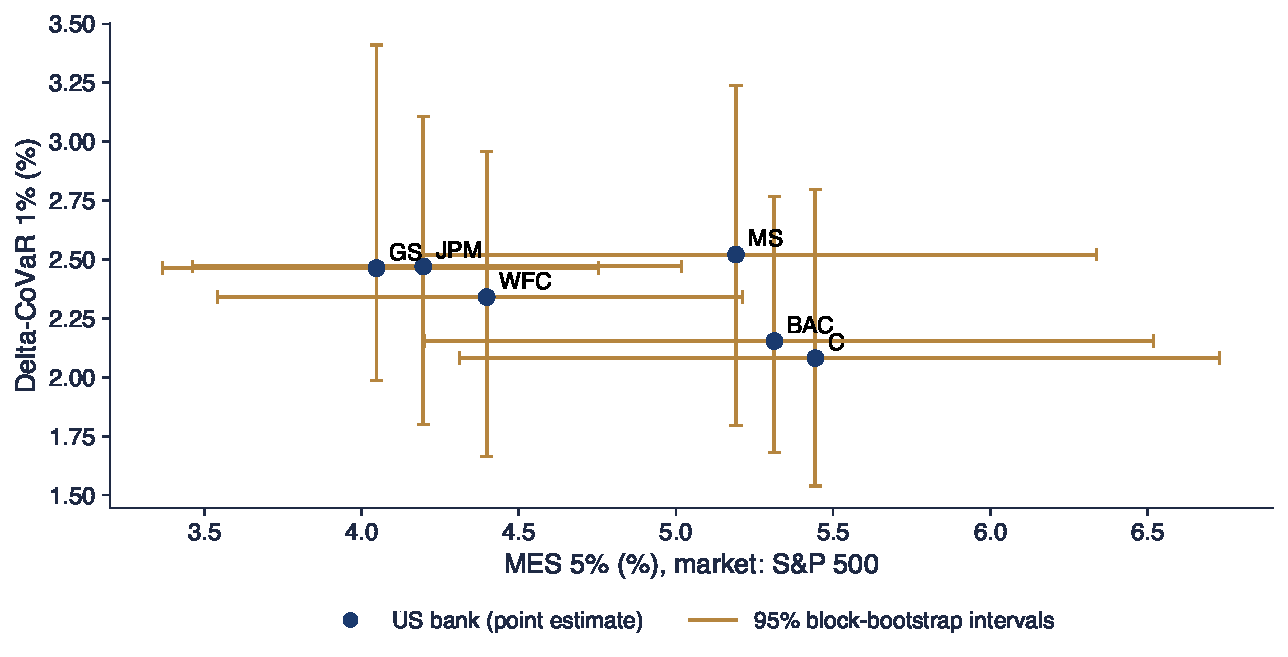
\includegraphics[width=0.96\textwidth,height=0.52\textheight,keepaspectratio]{ch15_sem_b1.pdf}
\end{center}
\vspace{-2mm}
\begin{itemize}
    \item $n = 5\,229$ days; largest MES: Citigroup; largest $\Delta$CoVaR: Morgan Stanley; Spearman correlation of the rankings $-0.60$
    \item Interpretation: no: MES ranks first the banks that fall most with the market (Citigroup, Bank of America), $\Delta$CoVaR the banks whose distress moves the market most; the intervals overlap, so neither ranking is sharp
\end{itemize}\sfmquantlet{Ch_15}{SFM_ch15_seminar}
\end{frame}

\begin{frame}{B2: European and Romanian Banks [Proposed]}
\itemsize{\footnotesize}
\begin{itemize}
\item \textbf{Question}: does the disagreement between MES and $\Delta$CoVaR found in B1 also appear in Europe and in Romania? Model: B1.
\item \textbf{Inputs}: five European banks and the Euro Stoxx 50 since 2005; TLV, BRD and the BET since 2010
\item \textbf{Tasks}
\begin{enumerate}
    \item Compute MES 5\% and $\Delta$CoVaR 1\% with bootstrap intervals for each bank, against its own market.
    \item Compute the Spearman correlation of the two rankings for the European banks.
    \item Compare the two Romanian banks on both measures.
    \item Interpretation: is the disagreement between MES and $\Delta$CoVaR as strong in Europe as in the US?
\end{enumerate}
\item \textbf{Report}: one table and two sentences
\item Notebook: section B2
\end{itemize}
\end{frame}

\ifsolutions
\begin{frame}{B2: Solution [Proposed]}
\itemsize{\footnotesize}
\begin{center}
\scriptsize
\begin{tabular}{lrrrr}
\toprule
& MES 5\% & 95\% interval & $\Delta$CoVaR 1\% & 95\% interval \\
\midrule
DBK & $4.81$ & [4.13, 5.49] & $2.90$ & [2.24, 3.83] \\
BNP & $4.60$ & [3.96, 5.29] & $3.13$ & [2.48, 3.67] \\
SAN & $4.35$ & [3.80, 4.95] & $3.09$ & [2.36, 3.82] \\
INGA & $5.35$ & [4.45, 6.33] & $3.18$ & [2.25, 3.90] \\
HSBA & $2.90$ & [2.47, 3.33] & $2.87$ & [2.14, 3.71] \\
\midrule
TLV & $3.54$ & [2.90, 4.24] & $3.31$ & [2.35, 4.78] \\
BRD & $3.00$ & [2.48, 3.70] & $3.05$ & [2.44, 4.12] \\
\bottomrule
\end{tabular}
\end{center}
\begin{itemize}
    \item Europe: largest MES ING, largest $\Delta$CoVaR ING; Spearman $0.70$; HSBC has by far the smallest MES
    \item Romania: TLV has the larger MES and $\Delta$CoVaR, but the intervals of the two banks overlap widely
    \item Interpretation: no: in Europe the two rankings agree much more than in the US; the banks are larger relative to the Euro Stoxx 50, so falling with the market and moving the market go together
\end{itemize}\sfmquantlet{Ch_15}{SFM_ch15_seminar}
\end{frame}
\fi

\begin{frame}{B3: US and European Banks in 2008 [Solved]}
\itemsize{\footnotesize}
\begin{itemize}
\item \textbf{Question}: did the link between US and European banks become stronger after Lehman: contagion or interdependence?
\item \textbf{Inputs}: equal-weighted portfolios of the six US and the five European banks, common days; calm: January 2005 -- June 2007; crisis: 15 September -- 31 December 2008
\item \textbf{Tasks}
\begin{enumerate}
    \item Compute the correlation of the two portfolios in the calm and in the crisis period.
    \item Test the rise in correlation with the one-sided Fisher $z$ test at 5\%.
    \item Compute $\delta$ from the variance of the US portfolio and the Forbes--Rigobon corrected correlation.
    \item Repeat the test with the corrected correlation.
    \item Interpretation: contagion or interdependence?
\end{enumerate}
\item \textbf{Report}: six numbers, two decisions, the chart and two sentences
\item Notebook: section B3
\end{itemize}
\end{frame}

\begin{frame}{B3: Solution [Solved]}
\itemsize{\scriptsize}
\begin{center}
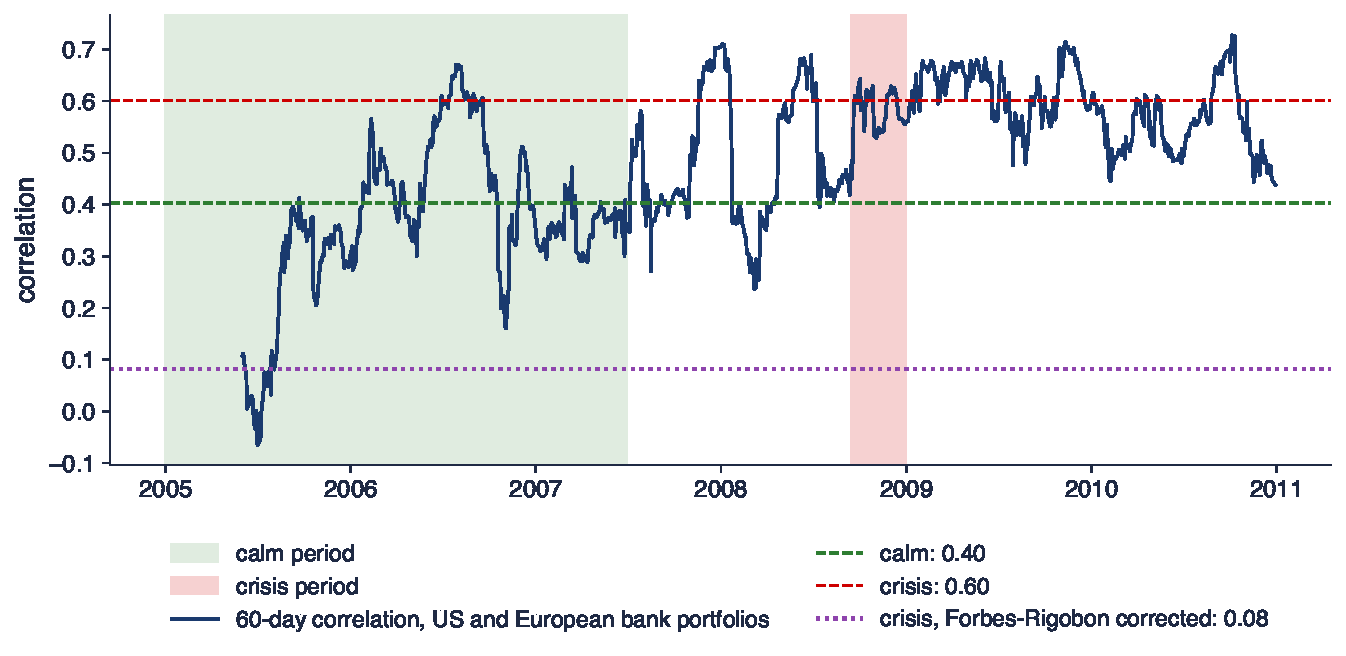
\includegraphics[width=0.96\textwidth,height=0.44\textheight,keepaspectratio]{ch15_sem_b3.pdf}
\end{center}
\vspace{-2mm}
\begin{itemize}
    \item $r_0 = 0.40$ ($n_0 = 506$), $r_1 = 0.60$ ($n_1 = 72$); $z = (0.695 - 0.428)/0.128 = 2.09$, p $= 0.018$: the raw rise is significant
    \item Variance of the US portfolio: $0.89$ $\to$ $75.39$, $\delta = 83.68$; $\rho^* = 0.60/\sqrt{1 + 83.68 \times 0.638} = 0.08$; $z = -2.69$, p $= 0.996$: no rise
    \item Interpretation: interdependence: the correlation rose because the variance of the US banks rose about 85 times; after the correction the link is not stronger \refFR
\end{itemize}\sfmquantlet{Ch_15}{SFM_ch15_seminar}
\end{frame}

\begin{frame}{B4: European and Romanian Banks in 2020 [Proposed]}
\itemsize{\footnotesize}
\begin{itemize}
\item \textbf{Question}: did the link between European and Romanian banks become stronger in the COVID-19 crash? Model: B3.
\item \textbf{Inputs}: equal-weighted portfolios of the five European banks and of TLV and BRD, common days since 2010; calm: 2019; crisis: 20 February -- 30 April 2020
\item \textbf{Tasks}
\begin{enumerate}
    \item Compute the correlation in the calm and in the crisis period and test the rise with the Fisher $z$ test.
    \item Compute $\delta$ from the variance of the European portfolio and the corrected correlation.
    \item Repeat the test with the corrected correlation.
    \item Interpretation: contagion or interdependence?
\end{enumerate}
\item \textbf{Report}: six numbers, two decisions and two sentences
\item Notebook: section B4
\end{itemize}
\end{frame}

\ifsolutions
\begin{frame}{B4: Solution [Proposed]}
\itemsize{\footnotesize}
\begin{itemize}
    \item $r_0 = 0.12$ ($n_0 = 200$), $r_1 = 0.70$ ($n_1 = 43$); $z = 4.29$, p $< 0.001$: the raw rise is significant
    \item Variance of the European portfolio: $2.50$ $\to$ $26.33$, $\delta = 9.52$; $\rho^* = 0.70/\sqrt{5.90} = 0.29$; $z = 1.03$, p $= 0.152$: not significant
    \item Interpretation: the evidence points to interdependence; with 2019 as the calm period the correlation was unusually low, and 43 crisis days give a wide interval, so the test has little power
\end{itemize}\sfmquantlet{Ch_15}{SFM_ch15_seminar}
\end{frame}
\fi

\begin{frame}{B5: Did MES in 2019 Rank the Losses of March 2020? [Solved]}
\itemsize{\footnotesize}
\begin{itemize}
\item \textbf{Question}: do the banks with a high MES before a crisis lose more in it, as in \refAPPR?
\item \textbf{Inputs}: 11 US and European banks; MES 5\% on the daily returns of 2019; buy-and-hold return from 19 February to 23 March 2020
\item \textbf{Tasks}
\begin{enumerate}
    \item Compute MES 5\% of each bank in 2019 against its own market.
    \item Compute the return of each bank from 19 February to 23 March 2020.
    \item Compute the Spearman correlation between MES and the return and its p-value.
    \item Interpretation: did MES rank the March 2020 losses?
\end{enumerate}
\item \textbf{Report}: the chart, the correlation with its p-value and two sentences
\item Notebook: section B5
\end{itemize}
\end{frame}

\begin{frame}{B5: Solution [Solved]}
\itemsize{\scriptsize}
\begin{center}
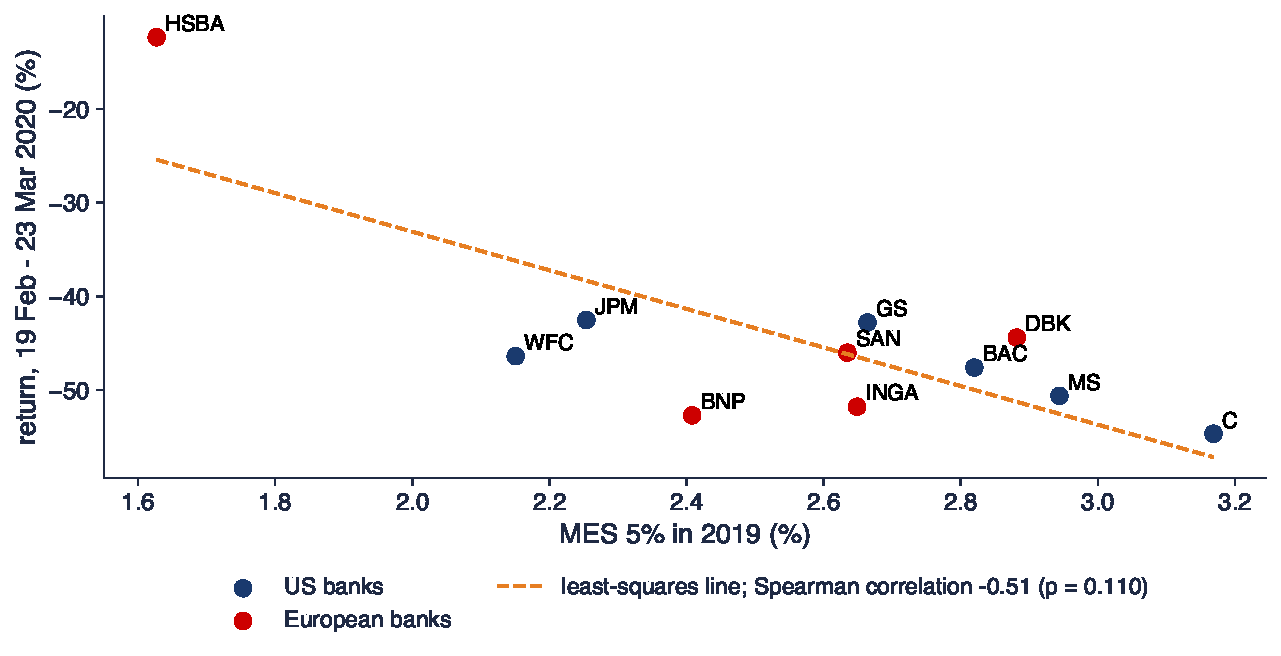
\includegraphics[width=0.96\textwidth,height=0.40\textheight,keepaspectratio]{ch15_sem_b5.pdf}
\end{center}
\vspace{-2mm}
\begin{itemize}
    \item Highest MES in 2019: Citigroup ($3.17\%$), also the worst return ($-54.7\%$); lowest MES: HSBC ($1.63\%$), also the smallest loss ($-12.3\%$)
    \item Spearman correlation $-0.51$, p $= 0.110$ ($n = 11$)
    \item Interpretation: partly: the sign is the one of \refAPPR{} and the extremes match, but with 11 banks the correlation is not significant at 5\%; the middle of the ranking is noise
\end{itemize}\sfmquantlet{Ch_15}{SFM_ch15_seminar}
\end{frame}

\begin{frame}{B6: Did MES in 2022 Rank the Losses of March 2023? [Proposed]}
\itemsize{\footnotesize}
\begin{itemize}
\item \textbf{Question}: does the result of B5 hold in the banking turmoil of March 2023? Model: B5.
\item \textbf{Inputs}: 13 banks (with TLV and BRD); MES 5\% on the daily returns of 2022; return from 28 February to 31 March 2023
\item \textbf{Tasks}
\begin{enumerate}
    \item Compute MES 5\% of each bank in 2022 against its own market.
    \item Compute the return of each bank from 28 February to 31 March 2023.
    \item Compute the Spearman correlation and its p-value.
    \item Interpretation: why may MES fail to rank the losses of March 2023?
\end{enumerate}
\item \textbf{Report}: one table, the correlation with its p-value and two sentences
\item Notebook: section B6
\end{itemize}
\end{frame}

\ifsolutions
\begin{frame}{B6: Solution [Proposed]}
\itemsize{\footnotesize}
\begin{center}
\scriptsize
\begin{tabular}{lrr|lrr}
\toprule
Bank & MES 5\% & return (\%) & Bank & MES 5\% & return (\%) \\
\midrule
JPM & $2.87$ & $-10.2$ & BNP & $4.71$ & $-16.5$ \\
BAC & $3.21$ & $-17.0$ & SAN & $4.21$ & $-8.0$ \\
C & $2.95$ & $-9.1$ & INGA & $5.43$ & $-17.6$ \\
GS & $2.90$ & $-8.0$ & HSBA & $2.56$ & $-13.5$ \\
MS & $3.41$ & $-10.8$ & TLV & $3.37$ & $-0.9$ \\
WFC & $3.28$ & $-20.1$ & BRD & $3.99$ & $-10.4$ \\
DBK & $5.20$ & $-20.7$ & & & \\
\bottomrule
\end{tabular}
\end{center}
\begin{itemize}
    \item Spearman $-0.35$, p $= 0.247$ ($n = 13$); highest MES: ING; worst return: Deutsche Bank
    \item Interpretation: the 2023 shock came from deposits and interest-rate risk at a few banks (SVB, Credit Suisse), not from a market crash: MES, built on market co-movement, ranks such a shock only weakly
\end{itemize}\sfmquantlet{Ch_15}{SFM_ch15_seminar}
\end{frame}
\fi


%=============================================================================
\section{Part C: Open Questions and AI Critique}
%=============================================================================

\begin{frame}{C1: How Connected Are Romanian and Euro-Area Banks? [Proposed]}
\itemsize{\footnotesize}
\begin{itemize}
\item \textbf{Question}: what share of the risk of TLV and BRD comes from the European banks, and does it rise in crises?
\item \textbf{Inputs}: the five European banks, TLV and BRD, daily log returns on common days since 2010; models: B1, the connectedness slide
\item \textbf{Tasks}
\begin{enumerate}
    \item Fit a VAR to the seven return series (order by BIC) and compute the connectedness table for $H = 10$ days.
    \item Compute the share of the forecast error variance of TLV and BRD that comes from the five European banks.
    \item Repeat it on rolling windows of 250 days and compare 2019 with 2020.
    \item Interpretation: is the systemic risk of the Romanian banks imported?
\end{enumerate}
\item \textbf{Report}: a table and a plan for a project
\item Notebook: section C1
\end{itemize}
\end{frame}

\ifsolutions
\begin{frame}{C1: Reference Analysis [Proposed]}
\itemsize{\footnotesize}
\begin{itemize}
    \item $n = 3\,245$ common days, VAR(1); total connectedness of the seven banks 60.0\%
    \item Share from the European banks, whole sample: TLV 22.9\%, BRD 22.1\%
    \item Rolling 250-day windows (average of TLV and BRD): mean 20.2\%, 2019 4.7\%, 2020 35.2\%, maximum 41.6\% (window ending 22 August 2022)
    \item Reading: in calm years almost all the risk of the Romanian banks is local; in crises a large share comes from the euro area
    \item Project design: different trading hours (two-day returns), $\Delta$CoVaR with the European bank portfolio as the conditioning variable, bootstrap intervals for the rolling shares
\end{itemize}\sfmquantlet{Ch_15}{SFM_ch15_seminar}
\end{frame}
\fi

\begin{frame}{C2: Audit an AI Answer [Proposed]}
\itemsize{\scriptsize}
\begin{itemize}
    \item A student asked an AI assistant to summarise the systemic risk of JPMorgan Chase. The answer:
    \item \aiprompt{(a) The CoVaR 99\% of the S\&P 500 given JPM is -4.80\%.}
    \item \aiprompt{(b) Delta-CoVaR = CoVaR - VaR of JPM = 4.80 - 6.27 = -1.48\%, so JPM reduces systemic risk.}
    \item \aiprompt{(c) MES 5\% is the average loss of the S\&P 500 on the worst 5\% of days of JPM.}
    \item \aiprompt{(d) The bank with the largest VaR 1\% is always the most systemic one.}
    \item \aiprompt{(e) The correlation of US and European banks rose from 0.40 to 0.60 in autumn 2008, which proves contagion.}
    \item \aiprompt{(f) A positive SRISK means that the bank has more capital than it needs in a crisis.}
    \item \aiprompt{(g) Granger causality from bank A to bank B means that past returns of A help to forecast B; it does not prove a causal channel.}
    \item Tasks
    \begin{itemize}
        \item 1. For each statement, say whether it is correct; if not, give the correct statement and, where possible, the correct number from the notebook (section C2).
        \item 2. Report: a list of seven verdicts with one line of justification each.
    \end{itemize}
\end{itemize}
\end{frame}

\ifsolutions
\begin{frame}{C2: Solution [Proposed]}
\itemsize{\footnotesize}
\begin{itemize}
    \item (a) Wrong twice: the level is the tail probability (CoVaR 1\%), and CoVaR is a loss, a positive number: CoVaR 1\% $= 4.80\%$
    \item (b) Wrong: $\Delta$CoVaR compares CoVaR in distress with CoVaR at the median of JPM: $\Delta$CoVaR 1\% $= 2.47\% > 0$ (A1)
    \item (c) Wrong: the conditioning is reversed: MES is the average loss of the bank on the market's worst days (A3)
    \item (d) Wrong: BAC has a larger VaR 1\% than JPM but a smaller $\Delta$CoVaR (A2)
    \item (e) Wrong: after the Forbes--Rigobon correction the crisis correlation is $0.08$: interdependence, not proven contagion (B3)
    \item (f) Wrong: SRISK $> 0$ is capital \textbf{missing} in a crisis; a surplus gives SRISK $< 0$ (A5)
    \item (g) Correct
\end{itemize}\sfmquantlet{Ch_15}{SFM_ch15_seminar}
\end{frame}
\fi


%=============================================================================
\section{Wrap-Up}
%=============================================================================

\begin{frame}{What You Should Take from Today}
\itemsize{\small}
\begin{itemize}
    \item CoVaR 1\% $= -(\hat a + \hat b\,q_{1\%}(X^i))$ and $\Delta$CoVaR $= \hat b\,(q_{50\%} - q_{1\%})$: the system given the bank
    \item MES: the bank given the market; SRISK $= kD - (1 - k)(1 - \mathrm{LRMES})W$ grows with leverage
    \item VaR, MES and $\Delta$CoVaR rank banks differently; rankings need bootstrap intervals
    \item A rise in correlation in a crisis is not proof of contagion: correct for volatility (Forbes--Rigobon)
    \item An AI answer is a draft: check the level, the sign, the direction of conditioning and the definition of $\Delta$CoVaR
\end{itemize}
\end{frame}

\begin{frame}{After the Seminar}
\itemsize{\small}
\begin{itemize}
    \item Lecture 15 develops each topic of today: the channels and the crises, CoVaR with state variables, MES and SRISK, networks, macroprudential policy
    \item Try the [Proposed] tasks in the notebook; the solutions are discussed in class
    \item C1 can grow into a team project: Romanian and euro-area banks, connectedness and $\Delta$CoVaR in 2011--2012, 2020 and 2023
    \item Reading: \refAB; \refAPPR; \refBE; survey: \refBCHP
\end{itemize}
\end{frame}


%=============================================================================
\section{References}
%=============================================================================

\begin{frame}{References}
\itemsize{\tiny}
\begin{itemize}
    \item Acharya, V.V., Engle, R., Richardson, M. (2012). \href{https://doi.org/10.1257/aer.102.3.59}{Capital shortfall: a new approach to ranking and regulating systemic risks}. \textit{American Economic Review}, 102(3), 59--64.
    \item Acharya, V.V., Pedersen, L.H., Philippon, T., Richardson, M. (2017). \href{https://doi.org/10.1093/rfs/hhw088}{Measuring systemic risk}. \textit{Review of Financial Studies}, 30(1), 2--47.
    \item Adrian, T., Brunnermeier, M.K. (2016). \href{https://doi.org/10.1257/aer.20120555}{CoVaR}. \textit{American Economic Review}, 106(7), 1705--1741.
    \item Benoit, S., Colliard, J.-E., Hurlin, C., Pérignon, C. (2017). \href{https://doi.org/10.1093/rof/rfw026}{Where the risks lie: a survey on systemic risk}. \textit{Review of Finance}, 21(1), 109--152.
    \item Brownlees, C., Engle, R.F. (2017). \href{https://doi.org/10.1093/rfs/hhw060}{SRISK: a conditional capital shortfall measure of systemic risk}. \textit{Review of Financial Studies}, 30(1), 48--79.
    \item Diebold, F.X., Yilmaz, K. (2012). \href{https://doi.org/10.1016/j.ijforecast.2011.02.006}{Better to give than to receive: predictive directional measurement of volatility spillovers}. \textit{International Journal of Forecasting}, 28(1), 57--66.
    \item Forbes, K.J., Rigobon, R. (2002). \href{https://doi.org/10.1111/0022-1082.00494}{No contagion, only interdependence: measuring stock market comovements}. \textit{Journal of Finance}, 57(5), 2223--2261.
    \item Franke, J., Härdle, W.K., Hafner, C.M. (2019). \href{https://doi.org/10.1007/978-3-030-13751-9}{\textit{Statistics of Financial Markets: An Introduction}}, 5th ed. Springer.
    \item Granger, C.W.J. (1969). \href{https://doi.org/10.2307/1912791}{Investigating causal relations by econometric models and cross-spectral methods}. \textit{Econometrica}, 37(3), 424--438.
    \item IMF, BIS, FSB (2009). \href{https://www.bis.org/publ/othp07.htm}{Guidance to assess the systemic importance of financial institutions, markets and instruments: initial considerations}. Report to the G-20 Finance Ministers and Central Bank Governors.
    \item Koenker, R., Bassett, G. (1978). \href{https://doi.org/10.2307/1913643}{Regression quantiles}. \textit{Econometrica}, 46(1), 33--50.
\end{itemize}
\end{frame}

\end{document}
